\chapter{Álgebra Lineal}

\section{Vectores}
El corazón del álgebra lineal son dos operadores, ambos con vectores;
Agreguemos vectores para conseguir $v+w$. Multiplicamos por los números $c$ y $d$ para conseguir
$cv$ y $dw$ Combinando las dos operaciones nos da una combinación linear\cite{strang1993introduction}.

\begin{equation}
	cv + dw = c\begin{bmatrix} 1 \\
		1\end{bmatrix} + d\begin{bmatrix} 2 \\
		3\end{bmatrix}=\begin{bmatrix} c+2d \\
		c+3d\end{bmatrix} \textup{Suma de vectores}.
\end{equation}

\begin{example}
	Tenemos la combinación con $c=d=1$
	\begin{equation*}
		c + d = \begin{bmatrix} 1 \\ 1 \end{bmatrix} + \begin{bmatrix} 2 \\ 3 \end{bmatrix}=\begin{bmatrix} 3\\ 4 \end{bmatrix}
	\end{equation*}
\end{example}

\subsubsection{Ideas clave}

Ahora definamos las tres ideas principales donde nos trasladaremos en el espacio n-dimensional:

\begin{enumerate}
	\item La suma de un vector $v+w$ y combinaciones lineares $cv+dw$.
	\item El producto escalar $x \cdot w$ de dos vectores y la longitud $\left\lVert v \right\rVert = \sqrt{v \cdot v}$.
	\item Matrices $A$, ecuaciones lineares $Ax=b$, soluciones $x=A^{-1}b$.
\end{enumerate}

La siguiente operación básica es la multiplicación escalar. Los vectores pueden ser multiplicados por cualquier número $c$
Hay dos formas de duplicar un vector; la primera es agregando el mismo $v+v$ y la más usual es multiplicando cada uno por dos.

\begin{equation}
	2v=\begin{bmatrix}
		2v_1\\
		2v_2 
	\end{bmatrix} \text{y también } -v= \begin{bmatrix}
		-v_1\\
		-v_2 
	\end{bmatrix}.
\end{equation}

\begin{example}
	Los componentes de $cv_{1}$ y $cv_2 $, el número $c$ es un escalar. Así que \textbf{la suma de $cv$ y $dw$ es una combinación linear
		de $v$ y $w$}.

	Calcular $v+w$

	\begin{equation*}
		v+w= \begin{bmatrix}
			4 \\
			2
		\end{bmatrix} + \begin{bmatrix}
			-1 \\
			2
		\end{bmatrix} = \begin{bmatrix}
			3 \\
			4
		\end{bmatrix}
	\end{equation*}

\end{example}

Multiplicación y adición al mismo tiempo en dos dimensiones $u+4v-2w$:
\begin{equation*}
	\begin{bmatrix} 1\\ 0\\ 3 \end{bmatrix}+4\begin{bmatrix} 1\\ 2\\ 1 \end{bmatrix}-2\begin{bmatrix} 2\\ 3\\ -1 \end{bmatrix}=\begin{bmatrix} 1\\ 2\\ 9 \end{bmatrix}
\end{equation*}
\begin{figure}[h!]
	\centerline{
\includegraphics[width=0.5\textwidth]{fal1.png}}
	\caption{ Representación gráfica de los vectores $v+w$}
	\label{fal1}
\end{figure}

Veamos a continuación algunos ejercicios:

\begin{problem}[Calcule $u + v +w$ y $2u + 2v + w$. ¿Dónde están $u,v,w$ en el plano?]
\begin{equation*}
	u=\begin{bmatrix} 1\\ 2\\ 3 \end{bmatrix} + v=\begin{bmatrix} -3\\ 1\\ -2 \end{bmatrix} + w=\begin{bmatrix} 2\\ -3\\ -1 \end{bmatrix} = \begin{bmatrix} 0\\ 0\\ 0 \end{bmatrix}
\end{equation*}
\end{problem}

\textit{ Sol. }
\begin{equation*}
	2\begin{bmatrix} 1\\ 2\\ 3 \end{bmatrix} + 2\begin{bmatrix} -3\\ 1\\ -2 \end{bmatrix} + \begin{bmatrix} 2\\ -3\\ -1 \end{bmatrix} = \begin{bmatrix} -2\\ 3\\ 1 \end{bmatrix}
\end{equation*}


\begin{problem}[Cada combinación de $v = (1, -2, 1)$ y $w = (0, 1, -1)$ tiene componentes que suman a ¿?. Encuentre $c$ y $d$ de modo que $cv + dw = (3,3, -6)$.]
\begin{align*}
	 & c\begin{bmatrix} 1\\ -2\\ 1 \end{bmatrix} + d\begin{bmatrix} 0\\ 1\\ -1 \end{bmatrix} = \begin{bmatrix} c\\-2c+d \\ c-d \end{bmatrix} \\
	 & c\begin{bmatrix} 1\\ -2\\ 1 \end{bmatrix} + d\begin{bmatrix} 0\\ 1\\ -1 \end{bmatrix} = \begin{bmatrix} 3\\ 3\\-6 \end{bmatrix}
\end{align*}
\end{problem}

\textit{ Sol. }

\begin{align*}
	 & c+0d  & =1  \\
	 & -2c+d & =3  \\
	 & c-d   & =-6
\end{align*}

Los componentes para todo $cv + dw$ suman cero. Resolviendo la última ecuación tenemos $C = 3$ y $d = 9$ quedando $(3,3, -6)$.

\begin{problem}[¿Qué punto del cubo es $i + j$? ¿Qué punto es la suma vectorial de $i = (1, 0, 0)$
y $j = (0,1,0)$ y $k = (0,0, I)$? Describe todos los puntos $(x, y, z)$ del cubo.]
\begin{equation*}
	\begin{bmatrix} 1\\ 0\\ 0 \end{bmatrix} + \begin{bmatrix} 0\\ 1\\ 0 \end{bmatrix} + \begin{bmatrix} 0\\ 0\\ 1 \end{bmatrix} = \begin{bmatrix} 1\\ 1\\ 1 \end{bmatrix}
\end{equation*}
\end{problem}

\textit{ Sol. }
\begin{figure}[h!]
	\centerline{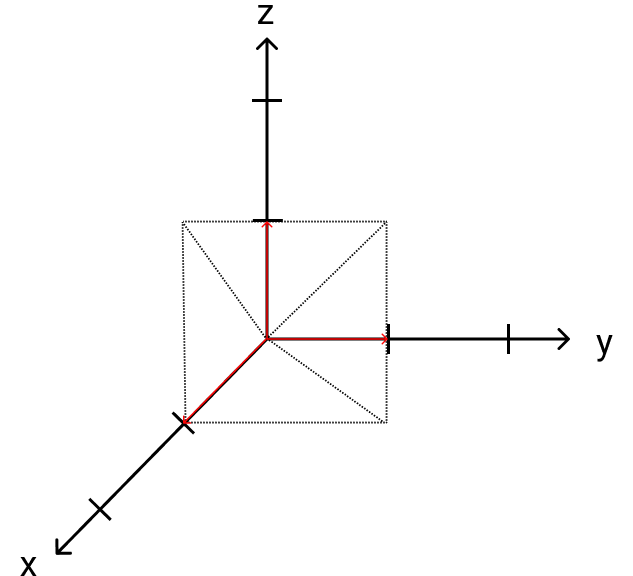
\includegraphics[width=0.3\textwidth]{fal2.png}}
	\caption{Los números en $c$ están igualmente separados en los tres ejes}
	\label{fal2}
\end{figure}

\begin{problem}[Las cuatro esquinas del cubo son $(0,0,0), (1,0,0), (0, 1,0), (0,0,1)$. ¿Cuáles son las otras cuatro esquinas? Encuentra las coordenadas del punto central del cubo. Cuáles son los puntos centrales
de las seis caras?]
\end{problem}

\textit{ Sol. }
definamos a $((1,0,0)$ como $i$, a $(0, 1,0)=j$ y $(0,0,1)=k$, entonces para encontrar todas las aristas faltantes tenemos que sumar $(i+j),(i+k),(j+k)$ e $(i+j+k)$

\begin{equation*}
	\begin{bmatrix} 1\\ 0\\ 0 \end{bmatrix} + \begin{bmatrix} 0\\ 1\\ 0 \end{bmatrix} = \begin{bmatrix} 1\\ 1\\ 0 \end{bmatrix}\ldots
\end{equation*}

Mientras que en los centros multiplicamos por: $\frac{1}{2}$:
\begin{equation*}
	\frac{1}{2}\begin{bmatrix} 1\\ 0\\ 0 \end{bmatrix} + \frac{1}{2}\begin{bmatrix} 0\\ 1\\ 0 \end{bmatrix}= \begin{bmatrix} \frac{1}{2}\\ \frac{1}{2}\\ 0 \end{bmatrix}\ldots
\end{equation*}

\begin{figure}[h!]
	\centerline{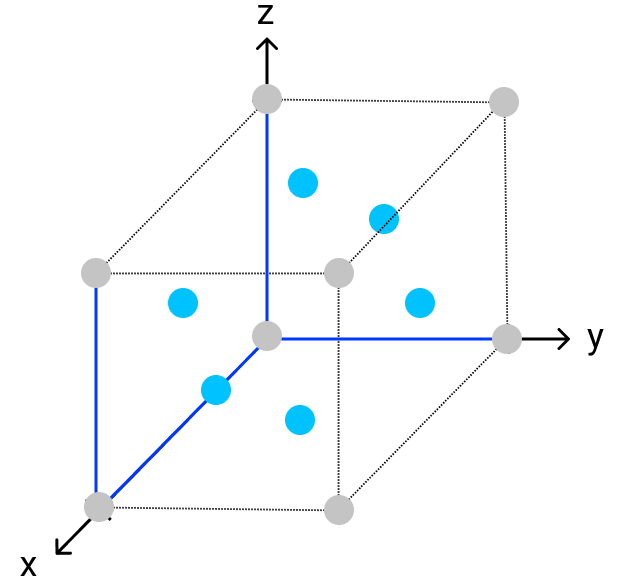
\includegraphics[width=0.3\textwidth]{fal3.png}}
	\caption{Cubo unitario desde i,j,k}
	\label{fal3}
\end{figure}

Las otras cuatro esquinas son $(1,1,0), (1,0,1), (0,1,1), (1,1,1)$. Los puntos céntricos son $(\frac{1}{2},\frac{1}{2}, \frac{1}{2})$.
Los centros de las caras son: $(\frac{1}{2}, \frac{1}{2}, 0), \left(\frac{1}{2}, \frac{1}{2}, 1\right)$ y $\left(0, \frac{1}{2}, \frac{1}{2}\right), \left(1, \frac{1}{2}, \frac{1}{2}\right)$ y $\left(\frac{1}{2}, 0, \frac{1}{2}\right), \left(\frac{1}{2}, 1, \frac{1}{2}\right)$.

\begin{problem}En la figura, muestra $\frac{1}{2}v + \frac{1}{2}w$. Marca los puntos $\frac{3}{4}v + \frac{1}{4}w$,
$\frac{1}{4}v + \frac{1}{4}w$ y $v+w$.
\end{problem}

\textit{ Sol. }

\begin{figure}[h!]
	\centerline{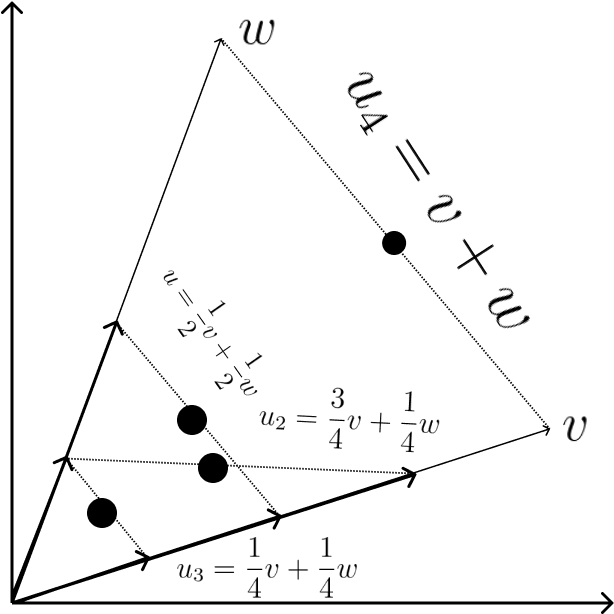
\includegraphics[width=0.3\textwidth]{fal4.png}}
	\caption{Puntos en los vectores}
	\label{fal4}
\end{figure}

\begin{problem}[Restringido solo por $c \geq 0$ y $d \geq 0$ dibuja el cono de todas las combinaciones $cv$ + $dw$.]
\end{problem}

\textit{ Sol. }
\begin{figure}[h!]
	\centerline{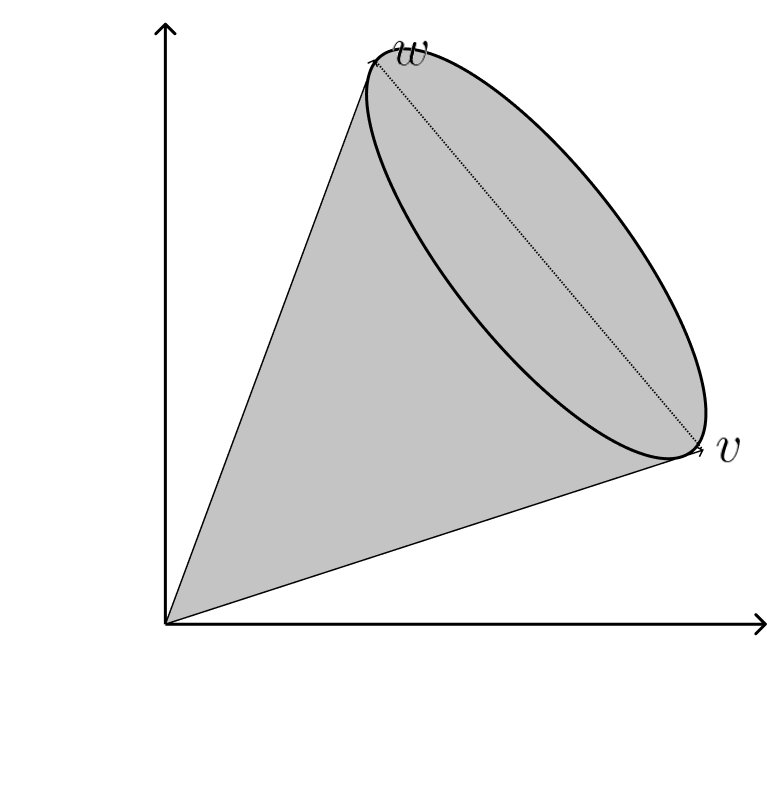
\includegraphics[width=0.3\textwidth]{fal5.png}}
	\caption{Cono}
	\label{fal5}
\end{figure}

\subsubsection{Longitud y producto punto}

\begin{definition}[Producto punto]
	El producto punto de $v= (v_{1},v_2 )$ y $w=(w_{1},w_2 )$
	es el número $v \cdot w$
\end{definition}

\begin{equation}
	v \cdot w = v_{1}w_1+ v_2 w_2 
\end{equation}

\begin{example}
	Los vectores $v=(4,2)$ y $w=(-1,2)$ tienen un producto punto cero:
	\begin{equation*}
		\begin{bmatrix} 4\\ 2 \end{bmatrix} \cdot \begin{bmatrix} -1\\ 2 \end{bmatrix}=-4+4=0
	\end{equation*}
\end{example}

Para este tipo de productos, el cero significa que estos dos vectores son perpendiculares.

\begin{equation}
	v\cdot w=0,
	\label{vecperpendicular}
\end{equation}

\subsubsection{Longitud y vectores unitarios}
Una caso importante es cuando los tenemos un vector dentro de un vector, en este caso $v$ es igual a $w$,
cuando el vector $v=(1+2+3)$ el producto punto con sigo mismo es $v \cdot v = \left\lVert v\right\rVert ^2  = 14 $

\begin{example}
	\[\left \| v \right \|^2 = \begin{bmatrix} 1\\ 2\\ 3 \end{bmatrix} \cdot \begin{bmatrix} 1\\ 2\\ 3 \end{bmatrix}=1+4+9=14\]
\end{example}

\begin{definition}[Longitud de un vector]
	La longitud $\left\lVert  v \right\rVert$ de un vector $v$ es igual a la raíz cuadrada de $v \cdot v$.
	\begin{equation}
		longitud= \left\lVert v \right\rVert = \sqrt{v \cdot v}
	\end{equation}
\end{definition}

\begin{definition}[vector unitario]
	un vector $u$ unitario es aquel que su longitud mide uno: $u\cdot u=1$
\end{definition}

Un vector unitario que va a la misma dirección que otro sería el siguiente: $u= \frac{v}{\left\lVert v\right\rVert }$. Ahora, como se mencionó en la
ecuación \ref{vecperpendicular}, nos forman un ángulo de 90$^{\circ}$, por lo que se nos forma un triángulo rectángulo
del cual derivamos ésta desigualdad

\begin{equation}
	\left | v \cdot w \right | \leqslant \left \| v \right \| \left \| w \right \|
\end{equation}

Si el ángulo formado es de 90$^{\circ}$ implica que el $\cos \theta=0$, ¿Qué nos dice ésto?, pues que si
el signo del producto punto $v \cdot v$ es positivo, entonces el ángulo $\theta$ es menor a 90$^{\circ}$ y homólogamente si es negativo
entonces el ángulo es mayor a 90$^{\circ}$.

Así es como llegamos a la fórmula \ref{formula_del_coseno}, la cual nos sirve cuando tenemos vectores que no son unitarios

\begin{equation}
	\textup{ Si $v$ y $w$ son dos vectores diferentes de cero, entonces} \frac{v\cdot w}{\left \| v \right \| \left \| w \right \|} = \cos \theta
	\label{formula_del_coseno}
\end{equation}

La idea principal la plantea la \textbf{desigualdad de Schwarz}, la cual dice que para cualquier ángulo,
el producto punto de $\frac{v}{\left\lVert v\right\rVert }$ con $\frac{w}{\left\lVert w\right\rVert }$
nunca excede de uno

\begin{equation}
	\textup{ Desigualdad de Schwarz } \left\lvert v \cdot 2\right\rvert  \leq \left\lVert v\right\rVert  \left\lVert w \right\rVert
\end{equation}

\begin{equation}
	\textup{ Desigualdad del triángulo } \left\lvert v+w \cdot 2\right\rvert  \leq \left\lVert v\right\rVert  + \left\lVert w \right\rVert
\end{equation}

\begin{example}
	El producto punto de $v \cdot w= 4$ ambos teniendo una longitud de $\sqrt{5} $.

	\begin{equation*}
		\cos \theta = \frac{4}{\sqrt{5} \sqrt{5}} = \frac{4}{5}
	\end{equation*}
\end{example}

\begin{problem}[Ahora veamos unos ejercicios:]
\begin{enumerate}
	\item Describa cada vector $w = (w_{1}, w_2 )$ que sea perpendicular a $v = (2, -1)$,
	\item Los vectores que son perpendiculares a $V = (1, 1, 1)$ se encuentran en ¿?,
	\item Los vectores que son perpendiculares a $(1, 1, 1)$ y $(1,2,3)$ se encuentran en ¿?
\end{enumerate}
\end{problem}

\textit{ Sol. }

\begin{enumerate}
	\item Todos los vectores $w = (c, 2c)$ son perpendiculares a $v$.
	\item Todos los vectores $(x, y, z)$ con $x + y + z = 0$
	      está en el plano.
	\item Todos los vectores perpendiculares a (1, 1, 1) y (1, 2, 3) se encuentran en una línea.
\end{enumerate}


\begin{problem}[Verdadero o falso]
(dé una razón si es verdadero o un contraejemplo si es falso)
\end{problem}


\begin{enumerate}
	\item Si $u$ es perpendicular (en tres dimensiones) a $v$ y $w$, esos vectores $v$ y $w$ son paralelos.
	\item Si $u$ es perpendicular a $v$ y $w$, entonces u es perpendicular a $v + 2w$,
	\item Si $u$ y $v$ son vectores unitarios perpendiculares, entonces $\left\lVert u-v\right\rVert = \sqrt{2} $
\end{enumerate}


\textit{ Sol. }

\begin{enumerate}
	\item [Falso] considerando $u=(1,0,0)$, $v=(0,1,0)$, $w=(0,0,1)$, no podrían ser paralelos porque significaría que irían a distintas direcciones.
	\item [Verdad] teniendo $u \cdot v = 0$ y $v \cdot w =0$ expandimos el producto $u\left(v+2w\right)$, Nos queda de la siguiente forma: $u\cdot 2w =2(u\cdot w) =2(0)$, como conclusión $u$ es ortogonal con $2w$.
	\item [Verdad] obtenemos la ecuación siguiente: $\sqrt{\left(u\right) \cdot \left(u\right)} =\left\lVert u-v\right\rVert$ sustituyendo $\sqrt{\left(1-1\right) \cdot \left(1-1\right)} = \sqrt{2}$
\end{enumerate}

\begin{problem}
Encuentre el ángulo $\theta$ (de su coseno) entre estos pares de vectores
\end{problem}

\begin{align}
	 & v=\begin{bmatrix} 1\\ \sqrt{3} \end{bmatrix} &  & y &  & w=\begin{bmatrix} 1\\ 0 \end{bmatrix}         \\
	 & v=\begin{bmatrix} 2\\ 2\\ -1 \end{bmatrix}   &  & y &  & w=\begin{bmatrix} 2\\ -1\\ 2 \end{bmatrix}    \\
	 & v=\begin{bmatrix} 1\\ \sqrt{3} \end{bmatrix} &  & y &  & w=\begin{bmatrix} -1\\ \sqrt{3} \end{bmatrix} \\
	 & v=\begin{bmatrix} 3\\ 1 \end{bmatrix}        &  & y &  & w=\begin{bmatrix} -1\\ -2 \end{bmatrix}
\end{align}
\textit{ Sol. }

\begin{enumerate}
	\item $\theta = \arccos \frac{1}{\left \| 2 \right \| \left \| 1 \right \|} = 60^{\circ}$
	\item $\theta = \arccos \frac{0}{\left \| 3 \right \| \left \| 3 \right \|} = 90^{\circ}$
	\item $\theta = \arccos \frac{2}{\left \| 2 \right \| \left \| 2 \right \|} = 60^{\circ}$
	\item $\theta = \arccos \frac{-5}{\left \| \sqrt{10} \right \| \left \| \sqrt{15} \right \|}= 135^{\circ}$
\end{enumerate}

\begin{problem}
Las pendientes de las flechas de $(0,0)$ a los puntos de $(v_{1}, v_2 )$ y $w_1/ w_2 $ son $v_2 /v_{1}$ y $w_2/ w_{1}$
Suponga que el producto $v_2 w_2/ v_1w_{1}$ de esas pendientes es $-1$. Muestre que $v \cdot w = 0$ y
que los vectores son perpendiculares.
\end{problem}

\textit{ Sol. }
Si $v_2 w_2 /v_{1}w_1= -1$ entonces $v_2w_2= -v_1w_{1}$ o $v_1w_1+ v_2w_2= v \cdot w = 0$: al dar 0, es perpendicular.

\begin{problem}
Con $v = (1, 1)$ y $w = (1, 5)$ elija un número $c$ de modo que $w - cv$ sea perpendicular
a $v$. Luego, encuentre la fórmula que dé este número $c$ para cualquier $v$ y $w$ distinto de cero.
(Nota: $cv$ es la ``proyección'' de $w$ sobre $v$.)
\end{problem}

\textit{ Sol. }

$\begin{bmatrix} 1\\ 5 \end{bmatrix} - c \begin{bmatrix} 1\\1 \end{bmatrix} = \begin{bmatrix} 1-c\\5-c \end{bmatrix}$

$(1,1)$ es perpendicular a $(1,5) - c (1, 1)$ si $(1-c)+(5-c)=6 - 2c = 0$ despejando, $c = 3$; $v \cdot (w - cv) = 0$ si
$c=v\cdot w / v\cdot v$. Restando $cv$ es la clave para los vectores perpendiculares.

\begin{problem}
La media geométrica de $x = 2$ y $y = 8$ es $\sqrt{XY}= 4$. La media aritmética es mayor:
$\frac{1}{2} (x + y) = ?$. Esto vendría en el ejemplo de la \textbf{desigualdad de Schwarz}
para $v = (\sqrt{2}, \sqrt{8})$ y $w = (\sqrt{8} , \sqrt{2} )$. Encuentre $\cos \theta $ para $v$ y $w$.
\end{problem}

\textit{ Sol. }

\begin{align*}
	 & \frac{1}{2} \left( x,y \right) = \frac{1}{2}(2+8)=5               \\
	 & u(\sqrt{2} ,\sqrt{8}), u(\sqrt{8},\sqrt{2} )                      \\
	 & \cos \theta = \frac{v \cdot w}{\left\lVert v \cdot w\right\rVert} \\
	 & \cos \theta = \frac{8}{\sqrt{10} \sqrt{10}} =\frac{8}{10}         \\
	 & \cos \theta = \frac{8}{10}
\end{align*}

\begin{problem}[El paralelogramo con lados $v = (4,2)$ y $w = (-1,2)$ es un rectángulo.]
Comprobar la
Fórmula de Pitágoras $a^2  + b^2  = c^2 $ que es solo para triángulos rectángulos:
\begin{quotation}
	(largo de $v$)$^2 $+(largo de $w$)$^2 $=(largo de $v+w$)$^2 $
\end{quotation}
\end{problem}

\textit{ Sol. }
\begin{align*}
	\centering
	 & (v)^2 +(w)^2 =(v+w)^2                                \\
	 & (\sqrt{20})^{\sqrt{5}}+(w)^2 =(\sqrt{20}+\sqrt{5})^2 \\
	 & 20+5=25                                              \\
	 & 25=25
\end{align*}

\subsection{Matrices}

Es un arreglo de números reales en filas y columnas. Con esto
será su tamaño, en general se refiere a filas por columnas. Cuando tiene el mismo número de filas es
una matriz cuadrada de orden $n$ y si son distintas son matrices rectangulares, existen triangulares superior e inferior, los cuales
se definen como una matriz que tenga ceros abajo y ceros arriba respectivamente:

\[\begin{bmatrix} 1 & 0 & 0\\ -1 & 1 & 0 \\ 0 &-1 & 1 \end{bmatrix} \begin{bmatrix} c\\ d\\ e \end{bmatrix}=\begin{bmatrix} c\\ d-c\\ e-d \end{bmatrix}\]

Esta es la interpretación $A \times x$ de la multiplicación de una matriz por un vector, véase que las columnas corresponden
a los componentes de los vectores. Podemos generalizar en la fórmula \eqref{eqcomblineal} como sigue:

\begin{equation}
	\label{eqcomblineal}
	Ax= \begin{bmatrix} u & v & w \end{bmatrix}\begin{bmatrix} c\\ d\\ e \end{bmatrix}= cu+dv+ew
\end{equation}

Así mismo existen las diferencias de matrices, finalmente una matriz por un vector nos genera un vector:
\begin{equation}
	Ax=\begin{bmatrix}
		1  & 0  & 0 \\
		-1 & 1  & 0 \\
		0  & -1 & 1
	\end{bmatrix}
	\begin{bmatrix}
		x_1\\
		x_2\\
		x_{3}
	\end{bmatrix}=
	\begin{bmatrix}
		x_1      \\
		x_2 -x_1\\
		x_{3}-x_2 
	\end{bmatrix}
\end{equation}

En el caso del producto punto, haciendo la combinación lineal ocurre la dinámica correspondiente:
\[Ax=\begin{bmatrix} 1 & 0 &0 \\ -1 & 1 &0 \\ 0 &-1 & 1 \end{bmatrix} \begin{bmatrix} x_{1}\\ x_2 \\ x_3 \end{bmatrix}= \begin{bmatrix} (1,0,0)\cdot (x_{1},x_2 ,x_{3}) \\ (-1,1,0)\cdot (x_{1},x_2 ,x_{3}) \\ (0,-1,1)\cdot (x_{1},x_2 ,x_{3}) \end{bmatrix}\]

\subsection{Ecuaciones lineales}
Recordemos que $x_{1},x_2 ,x_{3}$ no son cualquier incógnita, ya que estas contienen coordenadas;
La nueva dinámica será buscar $x$ con el resultado $b$. Para $Ax=b$ tenemos:

\begin{align*}
	 & x_1& =b_1            \\
	 & x_2& =b_{1}+b_2      \\
	 & x_3 & =b_{1}+b_2 +b_{3}
\end{align*}

Se puede simplificar se la siguiente forma:

\begin{equation}
	Ax= \begin{bmatrix} x_{1}\\ x_2 \\ x_3 \end{bmatrix}=\begin{bmatrix} b_1\\ b_{1}+b_2 \\ b_{1}+b_2 +b_3 \end{bmatrix} =\begin{bmatrix} 1 & 0 &0 \\ 1 & 1 &0 \\ 1 & 1 & 1 \end{bmatrix}\begin{bmatrix} b_{1}\\ b_2 \\ b_3 \end{bmatrix}
\end{equation}

Ahora, se observa una propiedad: \textbf{La suma de una matriz $S$, es la inversa de $A$}.

\begin{align*}
	 & Ax=\begin{bmatrix} 1 & 0 &0 \\ -1 & 1 &0 \\ 0 &-1 & 1 \end{bmatrix} \begin{bmatrix} 1\\ 2\\ 3 \end{bmatrix}= \begin{bmatrix} 1 \\ 1 \\ 1 \end{bmatrix} &  & Sb= \begin{bmatrix} 1 & 0 &0 \\ 1 & 1 &0 \\ 1 & 1 & 1 \end{bmatrix}\begin{bmatrix} 1 \\ 1 \\ 1 \end{bmatrix}=\begin{bmatrix} 1 \\ 2 \\ 3 \end{bmatrix}
\end{align*}

De aquí deducimos que: $Ax=b$ es resuelto por $x=A^{-1}b=Sb$.

\subsection{Diferencia cíclica}
Las combinaciones $u,v,w^*$ son una diferencia cíclica de la matriz $C$.
definamos.

\begin{align*}
	 & u=\begin{bmatrix} 1\\ -1\\ 0 \end{bmatrix}, v=\begin{bmatrix} 0\\ 1\\ -1 \end{bmatrix}, w^{*}=\begin{bmatrix} -1\\ 0\\ 1 \end{bmatrix}                                                               \\
	 & Cx=\begin{bmatrix} 1 & 0 &-1 \\ -1 & 1 &0 \\ 0 &-1 & 1 \end{bmatrix} \begin{bmatrix} x_{1}\\ x_2 \\ x_3 \end{bmatrix} = \begin{bmatrix} x_{1}-x_3 \\ x_2 -x_1\\ x_{3}-x_2\end{bmatrix}=b \\
\end{align*}

Ésta matriz $C$, no es triangular, en este caso es imposible encontrar $Cx=b$ porque puede haber infinitas soluciones o ninguna

\subsection{Dependencia e independencia lineal}

El punto importante es saber que $w*$ es una combinación lineal de $u$ y $v$:
\textbf{Dependencia:} $w$ no está en el plano de $u$ y $v$
\textbf{independencia linear:} $w^*$ está en el plano de $u$ y $v$.
\begin{align*}
	 & u+v+w^{*}=0 &  & w^{*}= \begin{bmatrix} -1\\ 0\\ 1 \end{bmatrix}=-u-v
\end{align*}

\subsubsection{Ideas clave}

\begin{enumerate}
	\item Matriz por el vector:$ Ax$= Combinación de las columnas de $A$
	\item La solución de Ax=b es $A^{-1}b$ cuando $A$ es una matriz invertible.
	\item La diferencia de la matriz $A$ es invertida por la suma de $S=A^{-1}$.
	\item La matriz cíclica $C$ no tiene inversa, sus tres columnas están en el plano.
	      Esas columnas dependientes suman cero al vector. $Cx=$0 tiene muchas soluciones.
\end{enumerate}

Ahora veamos unos ejercicios:
\begin{enumerate}
	\item Resuelve estas dos ecuaciones $Sy=b$ con $s_{1}, s_2 , s_{3}$ en las columnas de $s$:
	      \begin{align*}
		       & \begin{bmatrix} 1 & 0 &0 \\ 1 & 1 &0 \\ 1 & 1 & 1 \end{bmatrix}\begin{bmatrix} y_{1}\\ y_2 \\ y_3 \end{bmatrix} = \begin{bmatrix} 1\\ 1\\ 1 \end{bmatrix} &  & \begin{bmatrix} 1 & 0 &0 \\ 1 & 1 &0 \\ 1 & 1 & 1 \end{bmatrix}\begin{bmatrix} y_{1}\\ y_2 \\ y_3 \end{bmatrix} = \begin{bmatrix} 1\\4\\ 9 \end{bmatrix}
	      \end{align*}
	      \textit{ Sol. }

	      Las soluciones son $y_1= 1, y_2= 0, y_3 = 0$ (considerando al lado derecho como columna 1) e $y_1= 1, y_2= 3,
		      y_3 = 5$. Ese segundo ejemplo ilustra que los primeros $n$ números impares se suman a $n^2 $.

	\item Resuelva estas tres ecuaciones para $y_{1}, y_2 , y_{3}$ en términos de $B_{1}, B_2 , B_{3}$:
	      \begin{align*}
		      Sy & =B &  & \begin{bmatrix} 1 & 0 &0 \\ 1 & 1 &0 \\ 1 & 1 & 1 \end{bmatrix}\begin{bmatrix} y_{1}\\ y_2 \\ y_3 \end{bmatrix}= \begin{bmatrix} B_{1}\\ B_2 \\ B_3 \end{bmatrix}
	      \end{align*}
	      Escribe la solución y como una matriz $A = S^{-l}$ multiplicado por el vector $B$. ¿Son las columnas de S
	      independientes o dependientes?

	      \textit{ Sol. }
	      La combinación $Ow_1+ Ow_2+ Ow_{3}$ siempre da el vector cero, pero este problema
	      busca otras combinaciones de cero (entonces los vectores son dependientes, se encuentran en un plano):
	      $w_2= \frac{(w_1+ w_{3})}{2}$ entonces una combinación que da cero es $\frac{1}{2}W_1- W_2+ \frac{1}{2}W_{3}$

	\item Pasando a una ecuación de diferencia de 4 por 4 $Ax = b$, encuentre los cuatro componentes $x_{1}, x_2 ,
		      x_{3}, x_{4}$. Luego escribe esta solución como $x = Sb$ para encontrar la matriz inversa $S = A^{-1}$:
	      \begin{equation*}
		      Ax= \begin{bmatrix}
			      1  & 0  & 0  & 0 \\
			      -1 & 1  & 0  & 0 \\
			      0  & -1 & 1  & 0 \\
			      0  & 0  & -1 & 1
		      \end{bmatrix} \begin{bmatrix}
			      x_1\\
			      x_2\\
			      x_3 \\
			      x_{4}
		      \end{bmatrix}=\begin{bmatrix}
			      b_1\\
			      b_2\\
			      b_3 \\
			      b_{4}
		      \end{bmatrix}
	      \end{equation*}

	      \textit{ Sol. }

	      \begin{equation}
		      Sb= \begin{bmatrix}
			      1 & 0 & 0 & 0 \\
			      1 & 1 & 0 & 0 \\
			      1 & 1 & 1 & 0 \\
			      1 & 1 & 1 & 1\end{bmatrix}\begin{bmatrix}
			      b_1\\
			      b_2\\
			      b_3 \\
			      b_{4}
		      \end{bmatrix}= \begin{bmatrix}
			      x_1\\
			      x_2\\
			      x_3 \\
			      x_{4}
		      \end{bmatrix}
	      \end{equation}

	      \begin{align*}
		       & x_1& =b_1                   \\
		       & x_2& =b_{1}+b_2             \\
		       & x_3 & =b_{1}+b_2 +b_3        \\
		       & x_{4} & =b_{1}+b_2 +b_{3}+b_{4 }
	      \end{align*}
	      La primera columna de $A^{-1}$ es la solución para $b = (1,0,0,0)$. La segunda columna es la solución
	      para $b = (0,1,0,0)$. La tercera columna $x$ de $A^{-1}$ es la solución para $Ax = b = (0,0,1,0)$ y la cuarta columna $x$ de $A^{-1}$ es la solución para $Ax = b = (0,0,0,1)$.
	\item Una matriz de diferencias hacia adelante $\Delta$, es triangular superior:
	      \begin{equation*}
		      \Delta z= \begin{bmatrix} -1 & 1 &0 \\ 0 & -1 &1\\ 0 & 0 & -1 \end{bmatrix}\begin{bmatrix} z_{1}\\ z_2 \\ z_3 \end{bmatrix} = \begin{bmatrix} z_2 -z_{1}\\ z_{3}-z_2 \\ 0-z_3 \end{bmatrix} =\begin{bmatrix}
			      b_1\\b_2 \\b_{3}
		      \end{bmatrix}=b
	      \end{equation*}
	      Encuentre $z_{1}, z_2 , z_{3}$ a partir de $ b_{1},b_2 ,b_{3}$. ¿Cuál es la matriz inversa en $z= \Delta^{-1}b$?

	      \textit{ Sol. }
	      Se observa que en $b_{1}$ queremos encontrar a $z_{1}$, pero se encuentra en negativo: $b_{1}= z_2 -z_{1}$, así que para encontrar la matriz inversa se deben cambiar todos los signos como sigue en la ecuación:
	      \begin{equation}
		      z= \Delta^{-1}b= \begin{bmatrix} -1 & -1 &-1 \\ 0 & -1 &-1\\ 0 & 0 & -1 \end{bmatrix} \begin{bmatrix}
			      b_1\\b_2 \\b_{3}
		      \end{bmatrix} =\begin{bmatrix} z_{1}\\ z_2 \\ z_3 \end{bmatrix}
	      \end{equation}

	      \begin{align*}
		       & -z_2 +z_{1}-z_{3}+z_2 +z_{3}= = z_1\\
		       & -z_{3}+z_2 +z_{3}=z_2               \\
		       & z_{3}=z_{3}
	      \end{align*}
\end{enumerate}




\subsection{Resolución de sistemas de ecuaciones}

El problema central del álgebra lineal es resolver sistemas de ecuaciones.

\begin{center}
	\begin{tikzpicture}
		\draw[black,thick,->] (-2.5,0)--(5,0) node[right,below] {$x$}; % Eje x
		% Enumeración del eje x
		\foreach \x/\xtext in {-2/-2, -1/-1, 1/1, 2/2, 3/3, 4/4}
		\draw[shift={(\x,0)},black] (0pt,2pt)--(0pt,-2pt) node[below] {$\xtext$};
		%
		% Enumeración del eje y
		\foreach \y/\ytext in {-1/-1, 1/1, 2/2, 3/3, 4/4}
		\draw[shift={(0,\y)},black] (2pt,0pt)--(-2pt,0pt) node[left] {$\ytext$};
		\draw[black,thick,->] (0,-2)--(0,4.25) node[left,above] {$y$}; % Eje y
		%
		\node[below] at (-0.25,0){$O$};
		\draw[black,thick,<->] (0,-0.5) -- (5,2);
		\node[color=black,right] at (4,-1) {$x-2y=1$};
		%
		\draw[black,thick,<->] (0,5.5) -- (5,-2);
		\node[color=black,right] at (4,3) {$3x+2y=11$};
		%
		\draw[fill=black] (3,1) circle (2pt);
	\end{tikzpicture}
\end{center}


Las figura anterior muestra dos líneas que se encuentran en un punto, es esa intersección es la solución.
Si se quisiera representar como un vector, vamos a separarlo en columnas:

\begin{equation*}
	x\begin{bmatrix} 1\\ 3 \end{bmatrix}+y\begin{bmatrix} -2\\ 2 \end{bmatrix}=\begin{bmatrix} 1\\ 11 \end{bmatrix}b
\end{equation*}


Esto tiene dos vectores de columna en el lado izquierdo. El problema es encontrar la combinación de
Esos vectores que son iguales al vector de la derecha. Estamos multiplicando la primera columna por $x$
y la segunda columna por $y$, sumando con las opciones correctas: $x=3$ e $y=1$ ésto nos produce
$3(columna1)+1(columna2)=b$

La otra operación básica es la suma de vectores. Agregamos los primeros componentes y
segundos componentes por separado. La suma vectorial es $(1,11)$:

\begin{equation*}
	\begin{bmatrix} 3\\ 9 \end{bmatrix}+\begin{bmatrix} -2\\ 2 \end{bmatrix}=\begin{bmatrix} 1\\ 11 \end{bmatrix}
\end{equation*}

Para repetir: el lado izquierdo de la ecuación vectorial es una combinación lineal de las columnas.
El problema es encontrar los coeficientes correctos $x = 3$ e $y = 1$. Estamos combinando escalares,
multiplicación y suma de vectores en un solo paso. Ese paso es de vital importancia, porque
contiene las dos operaciones básicas:

\begin{equation*}
	3\begin{bmatrix} 1\\ 3 \end{bmatrix}+\begin{bmatrix} -2\\ 2 \end{bmatrix}=\begin{bmatrix} 1\\ 11 \end{bmatrix}
\end{equation*}

Por supuesto, la solución $x = 3$, $y = 1$ es la misma que en la imagen de la fila. las dos líneas que se cruzan son más familiares al principio.
La matriz de coeficientes en el lado izquierdo de las ecuaciones es la matriz $A$ de 2 por 2:

\begin{equation*}
	\text{matriz de coeficientes } A=\begin{bmatrix} 1& -2\\ 3& 2\end{bmatrix}
\end{equation*}

Esto es muy típico del álgebra lineal, mirar una matriz por filas y columnas. Sus filas
da la imagen de la fila y sus columnas da la imagen de la columna. Mismos números, diferentes
imágenes, mismas ecuaciones. Escribimos esas ecuaciones como un problema matricial $Ax = b$:

\begin{equation*}
	\text{}{Producto punto } A=\begin{bmatrix} 1& -2\\ 3& 2\end{bmatrix}\begin{bmatrix} x\\ y \end{bmatrix}=\begin{bmatrix} 1\\ 11 \end{bmatrix}
\end{equation*}


\subsubsection{Sistemas 3x3}

Las tres incógnitas son $x, y, z$. Tenemos tres ecuaciones lineales:

\begin{align*}
	   &    & x + 2y+ 3z=6 \\
	Ax & =b & 2x+5y+2z=4   \\
	   &    & 6x-3y+z=2
\end{align*}

Buscamos números $x, y, z$ que resuelvan las tres ecuaciones a la vez. Esos números deseados
podría o no existir. Para este sistema, existen. Cuando el número de incógnitas
coincide con el número de ecuaciones, por lo general hay una solución. Antes de resolver el problema,
lo visualizamos de ambas formas:

\begin{itemize}
	\item \textbf{Fila:} La imagen de la fila muestra tres planos que se encuentran en un solo punto.
	\item \textbf{Columna:} La imagen de la columna combina tres columnas para producir $(6,4,2)$.
\end{itemize}

La imagen de la columna comienza con la forma vectorial de las ecuaciones $Ax = b$:

\begin{equation*}
	\textit{Combinación de columnas} x\begin{bmatrix} 1\\2\\6 \end{bmatrix} +y\begin{bmatrix} 2\\5\\-3 \end{bmatrix}+z\begin{bmatrix} 3\\2\\1 \end{bmatrix}=\begin{bmatrix} 6\\4\\2 \end{bmatrix}
\end{equation*}

Las incógnitas son los coeficientes $x, y, z$. Queremos multiplicar los tres vectores de columna.
por los números correctos x, y, z para producir b = (6,4,2).


\section{Forma matricial de las ecuaciones}
Tenemos tres filas en la imagen de la fila y tres columnas en la imagen de la columna (más el
lado derecho). Las tres filas y las tres columnas contienen nueve números. Estos nueve números
llenan una matriz $A$ de 3 por 3:

\begin{equation*}
	A= \begin{bmatrix} 1&2&3\\2&5&2\\6&-3&1 \end{bmatrix}
\end{equation*}

La letra $A$ mayúscula representa los nueve coeficientes (en esta matriz cuadrada). La letra
$b$ denota el vector columna con componentes 6, 4, 2. La $x$ desconocida también es una columna
vector, con componentes $x, y, z$.  Por filas las ecuaciones eran (3), por columnas eran (4), y por matrices son (5):

\begin{equation*}
	\textit{Ecuación de la matriz} \begin{bmatrix} 1&2&3\\2&5&2\\6&-3&1 \end{bmatrix} \begin{bmatrix} x\\y\\z \end{bmatrix} = \begin{bmatrix} 6\\4\\2 \end{bmatrix}
\end{equation*}

¿Qué significa ``múltiplicar $A$ por $x$''? Podemos multiplicar por filas o
por columnas. De cualquier manera, $Ax = b$ debe ser una representación correcta de las tres ecuaciones.
De todas formas, haces las mismas nueve multiplicaciones.

$Ax$ proviene de productos escalares, cada fila multiplicada por la columna $x$:
\begin{equation}
	Ax= \begin{bmatrix} (fila1)\cdot x\\(fila2)\cdot x\\(fila3)\cdot x \end{bmatrix}
\end{equation}

La multiplicación por columnas $Ax$ es una combinación de vectores de columna:

\begin{equation}
	Ax= x\cdot (columna1) + y\cdot (columna1) + z\cdot (columna1)
\end{equation}

Cuando sustituimos la solución $x = (0,0,2)$, la multiplicación $Ax$ produce $b$:

\begin{equation*}
	\textit{Ecuación de la matriz} \begin{bmatrix} 1&2&3\\2&5&2\\6&-3&1 \end{bmatrix} \begin{bmatrix} 0\\0\\2 \end{bmatrix} = 1\times columna3 = \begin{bmatrix} 6\\4\\2 \end{bmatrix}
\end{equation*}

El producto escalar de la primera fila es $(1,2,3)\times (0,0,2) = 6$. Las otras filas dan punto
productos $4$ y $2$.

\subsubsection{Ideas clave}
\begin{enumerate}
	\item Las operaciones básicas sobre los vectores son la multiplicación $cv$ y la suma de vectores $v + w$.
	\item Juntas, esas operaciones dan combinaciones lineales $cv + dw$.
	\item Multiplicación matriz-vector Ax se puede calcular mediante productos escalares, una fila a la vez. Pero Ax debe entenderse como una combinación de las columnas de A.
	\item Imagen de columna: $Ax = b$ solicita una combinación de columnas para producir $b$.
	\item Imagen de fila: cada ecuación en Ax = b da una línea $(n = 2)$ o un plano $(n = 3)$ o un
	      "hiperplano" $(n> 3)$. Se cruzan en la solución o soluciones, si las hay.
\end{enumerate}
%%%%%%%%%%%%%%%%%%%%%%%%%%%%%%%%%%%
\subsubsection{Ejercicios de la forma matricial}
\begin{problem}[La primera de estas ecuaciones más la segunda es igual a la tercera:]
\begin{align*}
	 & x+ y+ z=2        \\
	 & x + 2y + z = 3   \\
	 & 2x + 3y + 2z = 5
\end{align*}
Los dos primeros planos se encuentran a lo largo de una línea. El tercer plano contiene esa línea, porque si $x, y, z$ satisfacen las dos primeras ecuaciones, entonces también la tercera pasa por esa línea. Las ecuaciones tienen infinitas soluciones (toda la \textbf{línea L}) Encuentra tres soluciones en L.
\end{problem}

\textit{ Sol. }
Se observa que existe una simetría entre fila, podemos obtener la solución sumando la primera columna con la segunda, la segunda con la tercera o la primera con la tercera.

\begin{equation}
	\begin{bmatrix}
		1 & 1 & 1 \\1&2&1\\ 2&3&2
	\end{bmatrix}\begin{bmatrix}
		1 \\1\\0
	\end{bmatrix} \text{ó} \begin{bmatrix}
		0 \\1\\1
	\end{bmatrix} \text{ó} \begin{bmatrix}
		1 \\0\\1
	\end{bmatrix} = \begin{bmatrix}
		2 \\3\\5
	\end{bmatrix}
\end{equation}

\begin{problem}[Mueva el tercer plano del problema 1 a un plano paralelo de $2x + 3y + 2z = 9$. Ahora las tres ecuaciones no tienen solución, ¿por qué no? Los dos primeros planos se encuentran a lo largo de la \textbf{línea L}, pero el tercer plano no tienen..? esa línea.]
\end{problem}

\textit{ Sol. }

La ecuación 1 + ecuación 2 - la ecuación 3 ahora es 0 = -4. La línea no pasa por el plano; no hay solución.

\begin{align}
	 & \begin{bmatrix}
		   1 & 1 & 1 \\1&2&1\\ -2&-3&-2
	   \end{bmatrix}\begin{bmatrix}
		                1 \\1\\1
	                \end{bmatrix} = \begin{bmatrix}
		                                0 \\0\\0
	                                \end{bmatrix} \\
	 & \begin{bmatrix}
		   1 & 1 & 1 \\1&2&1\\ -2&-3&-9
	   \end{bmatrix}\begin{bmatrix}
		                1 \\1\\1
	                \end{bmatrix} = \begin{bmatrix}
		                                0 \\0\\-4
	                                \end{bmatrix}
\end{align}

\begin{problem}[Calcule cada eje del problema como una combinación de las columnas:]
\begin{equation*}
	Ax= 2\begin{bmatrix}
		1 \\-2\\-4
	\end{bmatrix}+2\begin{bmatrix}
		2 \\3\\1
	\end{bmatrix}+3\begin{bmatrix}
		4 \\1\\2
	\end{bmatrix}=\begin{bmatrix}
		 & \\ & \\&
	\end{bmatrix}
\end{equation*}
¿Cuántas multiplicaciones separadas para $Ax$, cuando la matriz es 3 por 3?
\end{problem}

\textit{ Sol. }

Aplicando el producto punto en las columnas y luego sumar, el resultado de la matriz es:
\begin{equation*}
	Ax= 2\begin{bmatrix}
		1 \\-2\\-4
	\end{bmatrix}+2\begin{bmatrix}
		2 \\3\\1
	\end{bmatrix}+3\begin{bmatrix}
		4 \\1\\2
	\end{bmatrix}=\begin{bmatrix}
		18 \\5\\0
	\end{bmatrix}
\end{equation*}

\begin{problem}
	\begin{enumerate}
		\item  Una matriz con $m$ filas y $n$ columnas multiplica un vector con \dots ? componentes para producir un vector con \dots ? componentes.
		\item Los planos de las $m$ ecuaciones $Ax = b$ son en el espacio dimensional.
		La combinación de las columnas de $A$ es un espacio en \dots? dimensiones.
	\end{enumerate}
\end{problem}

\textit{ Sol. }

\begin{enumerate}
	\item un vector de $n$ columnas
	\item con $m$ combinaciones de posibles vectores
	\item $n$ dimensiones
	\item $m$ dimensiones
\end{enumerate}

\begin{problem}[¿Qué matriz $E$ de 2 por 2 resta el primer componente del segundo componente?
¿Qué matriz de 3 por 3 hace lo mismo?]
\begin{align*}
	 & E\begin{bmatrix} 3\\5 \end{bmatrix}= \begin{bmatrix} 3\\2 \end{bmatrix} &  & E\begin{bmatrix} 3\\5\\7 \end{bmatrix}= \begin{bmatrix} 3\\2\\7 \end{bmatrix}
\end{align*}
\end{problem}

\textit{ Sol. }

\begin{equation*}
	E= \begin{bmatrix} 1 & 0\\-1 & 1\end{bmatrix},E= \begin{bmatrix} 1 & 0&0\\-1 & 1&0 \\ 0&0&1 \end{bmatrix}
\end{equation*}
Se obtienen restando el primer componente del segundo.

\begin{problem}
¿Qué matriz $R$ de 2 por 2 rota cada vector $45^{\circ}$? El vector (1,0) va a
$(\frac{\sqrt{2}}{2}, \frac{\sqrt{2}}{2})$. El vector (0, 1) va a $(-\frac{\sqrt{2}}{2},\frac{\sqrt{2}}{2})$. Esos determinan la matriz. Dibuje estos vectores particulares en el plano $xy$ y encuentre $R$.
\end{problem}

\textit{ Sol. }

\begin{center}
	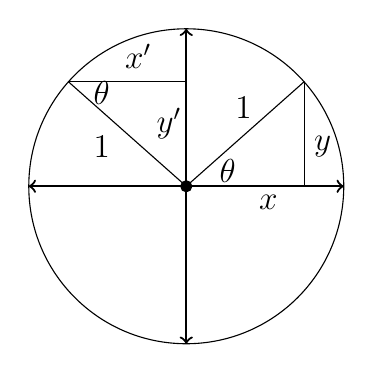
\begin{tikzpicture}
		\draw (1,1) circle (2);
		\draw [fill] (1,1) circle (0.07);
		\draw [-] (1,1)-- (2.5,1);
		\draw [-] (2.5,1)-- (2.5,2.33);
		\draw (1,1)-- (2.5,2.33);
		\draw [-] (1,1)-- (1,2.33);
		\draw (1,2.33)-- (-0.5,2.33);
		\draw (-0.5,2.33) to (1,1);
		\draw [<->,thick] (-1,1) to (3,1);
		\draw [<->,thick] (1,-1) to (1,3);
		\node[right] at (2.5,1.5){\large $y$};
		\node[right] at (1.5,2){\large $1$};
		\node[right] at (1.8,0.8){\large $x$};
		\node[right] at (1.3,1.2){\large $\theta$};
		\node[right] at (0.5,1.8){\large $y^{\prime}$};
		\node[right] at (-0.3,1.5){\large $1$};
		\node[right] at (0.1,2.65){\large $x^{\prime}$};
		\node[right] at (-0.3,2.18){\large $\theta$};
	\end{tikzpicture}
	\begin{align*}
		\cos{\theta} & =\frac{x}{1}                  & \sin{\theta} & =\frac{y}{1}                                                                                      \\
		R_{\theta}   & =\begin{bmatrix}
			                x \\ y
		                \end{bmatrix}=\begin{bmatrix}
			                              \cos{\theta} \\ \sin{\theta}
		                              \end{bmatrix} & R_{\theta}   & =\begin{bmatrix}
			                                                              x \\ y
		                                                              \end{bmatrix}=\begin{bmatrix}
			                                                                            \cos{\theta} \\ \sin{\theta}
		                                                                            \end{bmatrix}=\begin{bmatrix}
			                                                                                          \frac{\sqrt{2}}{2} \\ \frac{\sqrt{2}}{2}
		                                                                                          \end{bmatrix}
	\end{align*}
\end{center}

Finalmente, se construye un triángulo con la proyección al cuadrante II,
y planteamos lo siguiente:
\begin{align*}
	R_{\theta}=\begin{bmatrix}
		           -\sin{\theta} \\ \cos{\theta}
	           \end{bmatrix} \implies                                                                                          & R_{45^{o}}=\begin{bmatrix}
		                                                                                                                                        0 \\ 1
	                                                                                                                                        \end{bmatrix}= \begin{bmatrix}
		                                                                                                                                                       -\sin{\theta} \\ \cos{\theta}
	                                                                                                                                                       \end{bmatrix}      \\
	R_{\theta}= \begin{bmatrix}
		            \frac{1}{\sqrt{2}} & \frac{-1}{\sqrt{2}} \\ \sqrt{2} & \frac{1}{\sqrt{2}}
	            \end{bmatrix} & = \begin{bmatrix}
		                              \cos{45^{o}} & -\sin{45^{o}} \\ \sin{45^{o}} & \cos{45^{o}}
	                              \end{bmatrix}
\end{align*}
Una vez obtenidos los valores, procedemos a graficar:

\begin{center}
	\begin{tikzpicture}
		\draw [color=blue, ->] (0,0) to (2.5,1.5) node[right] {$\begin{bmatrix}
					\frac{1}{\sqrt{2}} \\ \frac{1}{\sqrt{2}}
				\end{bmatrix}$};
		\draw [color=blue, ->] (0,0) to (-2.5,1.5) node[left] {$\begin{bmatrix}
					-\frac{1}{\sqrt{2}} \\ \frac{1}{\sqrt{2}}
				\end{bmatrix}$};
		\draw [color=red,->,thick] (0,0) -- (1.75,0) node[below] {$\begin{bmatrix}
					1 \\ 0
				\end{bmatrix}$};
		\draw [color=red,->,thick](0,0) to (0,2) node[left] {$\begin{bmatrix}
					0 \\ 1
				\end{bmatrix}$};
		\draw[<->] (-2.5,0) -- (2.5,0) node[right]{x};
		\draw[<->] (0,-1) -- (0,2.5) node[right]{y};
	\end{tikzpicture}
\end{center}

\begin{problem}
Los comandos de \texttt{MATLAB} $A = eye (3)$ y $v = [3: 5]^{\prime}$ producen la matriz identidad de 3 por 3
y el vector columna (3, 4, 5) ¿Cuáles son las salidas de $A * v$ y $v^{\prime} * v$?
(¡No se necesita computadora!) Si solicita $v * A$, ¿qué sucede?
\end{problem}

\textit{ Sol. }
Después de poner el código en \texttt{MATLAB}, obtenemos:
\begin{equation}
	A= \begin{bmatrix}
		1 & 0 & 0 \\0&1&0\\0&0&1
	\end{bmatrix}, \quad v=\begin{bmatrix}
		3 \\4\\5
	\end{bmatrix}
\end{equation}
donde $A$ es una matriz identidad de 3x3, y la columna $v$ es un vector. Expresemos a $v^{\prime}$ como una columna de vectores transpuestos:
\begin{align*}
	A\cdot v= \begin{bmatrix}
		             1 & 0 & 0 \\0&1&0\\0&0&1
	             \end{bmatrix}\cdot \begin{bmatrix}
		                                3 \\4\\5
	                                \end{bmatrix}=\begin{bmatrix}
		            1\cdot 3+0\cdot4+0\cdot5   \\
		            0\cdot 3+1\cdot 4+0\cdot 5 \\
		            0\cdot 3+0\cdot 4+1\cdot 5
	            \end{bmatrix}=\begin{bmatrix}
		            3 \\4\\5
	            \end{bmatrix}=v
\end{align*}
Ahora consideremos el producto $v\cdot v^{\prime}$
\begin{equation*}
	v\cdot v^{\prime}= \begin{bmatrix}
		3 & 4 & 5 \\
	\end{bmatrix}\cdot \begin{bmatrix}
		3 \\4\\5
	\end{bmatrix}=50
\end{equation*}

El número de columnas en la matriz $v$ es una, cual no es el mismo número de filas en la matriz $A$, que tiene tres; En ese caso no se puede determinar su producto.
\begin{align}
	 & A\cdot v          & =v                                 \\
	 & v^{\prime}\cdot v & =50                                \\
	 & v\cdot A          & \quad \text{No existe el producto}
\end{align}

\begin{problem}
Comienza con el vector $U_{0} = (1,0)$. Multiplica una y otra vez por el mismo ``matriz de Markov'' $A = [{.}8{.}3; {.}2{.}7]$. Los siguientes tres vectores son $u_{1}, u_2 , u_{3}$
\begin{equation*}
	u_{1}= \begin{bmatrix} {.}8 & {.}3\\{.}2 & {.}7 \end{bmatrix}\begin{bmatrix} 1\\0 \end{bmatrix}= \begin{bmatrix} {.}8\\{.}2 \end{bmatrix}, \quad u_2 =Au_{1}=?, \quad u_{3}=Au_2 =?
\end{equation*}
\end{problem}

\textit{ Sol. }
\begin{equation*}
	u_2 =\begin{bmatrix} {.}8 & {.}3\\{.}2 & {.}7 \end{bmatrix}\cdot \begin{bmatrix} {.}8\\{.}2 \end{bmatrix}= \begin{bmatrix} {.}7\\{.}3 \end{bmatrix}
\end{equation*}
\begin{equation*}
	u_{3}=\begin{bmatrix} {.}8 & {.}3\\{.}2 & {.}7 \end{bmatrix}\cdot \begin{bmatrix} {.}7\\{.}3 \end{bmatrix}= \begin{bmatrix} {.}65\\{.}35 \end{bmatrix}
\end{equation*}
Se observa que tanto los vectores $u_{0},u_{1},u_2 ,u_{3}$ Siempre suman uno.

\begin{problem}
Continúe con el problema 29 de $u_{0} = (1,0)$ a $u_{7}$, y también de $v_{0} = (0,1)$ a $v_{7}$.
¿Qué observa acerca de $u_{7}$ y $v_{7}$? Aquí hay dos códigos \texttt{MATLAB}, con \textbf{while} y
\textbf{for}. Trazan $u_{0}$ a $u_{7}$ y $v_{0}$ a $v_{7}$. Puede utilizar otros idiomas:
\end{problem}

\textit{ Sol. }
$U7$, $V7$, $W7$ están todos cerca de (0.6, 0.4). Sus componentes aún se suman a 1.

\begin{notation}
	De las matrices:

	La primera fila de una matriz de 2 por 2 contiene $a_{11}$ y $a_{12}$. La segunda fila contiene $a_{21}$ y
	$a_{22}$. El primer índice da el número de fila, de modo que $a_{ij}$ es una entrada en la fila $i$. El segundo índice
	$j$ da el número de columna. ¡Pero esos subíndices no son muy convenientes en un teclado!
	En lugar de $aU$ escribimos$A (i, j)$. La entrada $a_{57}$ = $A (5, 7)$ estaría en la fila 5, columna 7.
	\begin{equation}
		A= \begin{bmatrix}
			a_{11} & a_{12} \\
			a_{21} & a_{22}
		\end{bmatrix}
	\end{equation}
\end{notation}


Para una matriz de $m$ por $n$, el índice de fila $i$ va de $1$ a$ m$. El índice de columna $j$ se detiene en $n$.
Hay $mn$ entradas $a_{ij} = A (i, j)$. Una matriz cuadrada de orden $n$ tiene $n^2 $ entradas.

\subsection{Eliminación}
Es una forma sistemática de resolver ecuaciones lineales. Por ejemplo:
\begin{align*}
	\text{Antes$\ldots$} x-2y & =1   & \text{Después$\ldots$} x-2y & =1 \\
	3x + 2y                   & = 11 & 8y                          & =8
\end{align*}

La nueva ecuación $8y=8$ da instantáneamente $y = 1$. Sustituyendo $y = 1$ nuevamente en la primera
la ecuación deja $x-2 = 1$. Por lo tanto, $x = 3$ y la solución $(x, y) = (3, 1)$ está completa.

La eliminación produce un \textbf{sistema triangular superior}: este es el objetivo.

\begin{definition}[Pivote]
	Primer no cero en la fila que produce la eliminación
\end{definition}

\begin{definition}[Multiplicador]
	Es la entrada para eliminar el pivote.
\end{definition}

Para resolver $n$ ecuaciones queremos $n$ pivotes. Los pivotes están en la diagonal del triángulo después de la eliminación.

\subsubsection{Desglose de la eliminación}

Normalmente, la eliminación produce los pivotes que nos llevan a la solución. Pero el fracaso es posible. En algún momento, el método puede pedirnos que dividamos por cero. No podemos hacerlo. El proceso
tiene que detenerse. Puede haber una manera de adaptarse y continuar, o el fracaso puede ser inevitable.

\begin{definition}[Fallas]
	Para $n$ ecuaciones no obtenemos $n$ pivotes, se puede tener ninguna o infinitas soluciones y por último, que el pivote sea igual a cero, aunque se puede arreglar haciendo una permutación en las filas.
\end{definition}

\subsubsection{Eliminación gaussiana}

\begin{align*}
	 & 2+4y-2z=2    \\
	 & 4x+9y-3z8    \\
	 & -2x-3y+7z=10
\end{align*}

\begin{enumerate}
	\item Paso 1: Reste 2 veces la ecuación 1 de la ecuación 2. Esto deja $y + z = 4.$
	\item Paso 2: Reste -1 por la ecuación 1 de la ecuación 3. Esto deja $y + 5z = 12$.
	      Las dos nuevas ecuaciones involucran solo $y$ y $z$. El segundo pivote es 1:
	      \begin{align*}
		       & 1y+1z=4  \\
		       & 1y+5z=12
	      \end{align*}

	\item Paso 3: Reste la nueva ecuación 2 de la nueva 3. El multiplicador es $1/1 = 1$. Luego $4z = 8$.
	      El $Ax = b$ original se ha convertido en un triangular superior $Ux=c$:

	      \begin{align*}
		      2+4y-2z   & =2  & 2+4y-2z & =2  \\
		      4x+9y-3z  & =8  & 1y+1z   & =4  \\
		      -2x-3y+7z & =10 & 4       & z=8
	      \end{align*}
	\item Paso 4: El objetivo se logró: la eliminación hacia adelante se completa de $A$ a $U$. Observe los pivotes
	      2, 1,4 a lo largo de la diagonal de U. Los pivotes 1 y 4 estaban ocultos en el sistema original.
	      La eliminación los sacó. $Ux = c$ está listo para la sustitución. La solución es $(x, y, z) = (-1,2,2)$.
\end{enumerate}

La imagen de la columna muestra una combinación $Ax$ de vectores de columna que producen la derecha
lado b. Los coeficientes en esa combinación son -1,2,2 (la solución):

\begin{equation*}
	Ax= -1\begin{bmatrix}
		2 \\4\\-2
	\end{bmatrix}+2 \begin{bmatrix}
		4 \\9\\-3
	\end{bmatrix}+2 \begin{bmatrix}
		-2 \\-3\\7
	\end{bmatrix}= \begin{bmatrix}
		2 \\8\\10
	\end{bmatrix}=b
\end{equation*}

\subsubsection{Ideas clave}

\begin{enumerate}
	\item Un sistema lineal ($Ax = b$) se convierte en triangular superior ($Ux = c$) después de la eliminación.
	\item Restamos $l_{ij}$ multiplicado por la ecuación $j$ de la ecuación $i$, para hacer que la entrada $(i, j)$ sea cero.
	\item El multiplicador es $l_{ij}=\frac{\text{Entrada para eliminar en la fila i}}{\text{pivote en la columna j}}$. Los pivotes no pueden ser cero.
	\item Un cero en la posición de pivote se puede reparar si hay un valor distinto de cero debajo de él.
	\item El sistema triangular superior se resuelve mediante sustitución hacia atrás (comenzando por la parte inferior).
	\item Cuando la avería es permanente, el sistema no tiene solución o es infinita.
\end{enumerate}

\subsection{Eliminación usando matrices}

Ahora combinamos dos ideas: eliminación y matrices. El objetivo es expresar todos los pasos.
de eliminación (y el resultado final) de la forma más clara posible. En un ejemplo de 3 por 3,
la eliminación podría describirse con palabras. Para sistemas más grandes, una larga lista de pasos sería
sin esperanza. Verá cómo restar un múltiplo de la fila $j$ de la fila $i$ utilizando una matriz $E$.

Esta regla para $Ax$ se usa con tanta frecuencia que la expresamos una vez más para dar énfasis.

$Ax$ es una combinación de las columnas de $A$ Los componentes de $x$ en esas columnas:

\begin{equation}
	Ax= x_{1}\times (\text{Columna 1})+x_2 \times (\text{Columna 2})+\cdots+x_{n}\times (\text{Columna $n$})
\end{equation}

\begin{notation}
	La fórmula corta para ese producto escalar con $x$ usa ``notación sigma''.
	Los componentes de $Ax$ son productos escalares con filas de $A$.

	\begin{equation}
		Ax= a_{ix1}x_{1}+ a_{ix2}x_2 +\cdots +a_{ixn}x_{n} = \sum_{j=1}^{n} a_{ij}x_{j}
	\end{equation}
\end{notation}

\subsubsection{La forma matricial de un paso de eliminación}

Queremos hacer esa resta con una matriz, Se logra el mismo resultado con $b_{n} = E_{b}$
cuando multiplicamos una ``matriz de eliminación'' $E$ por $b$. Resta $2b_{1}$ de $b_2 $:

\begin{equation}
	\text{Matriz de eliminación } E=\begin{bmatrix}
		1 & 0 & 0 \\ -2& 1& 0 \\ 0 &0 &1
	\end{bmatrix}
\end{equation}

La multiplicación por $E$ resta 2 veces la fila 1 de la fila 2. Las filas 1 y 3 permanecen iguales:

\begin{equation}
	\begin{bmatrix}
		1 & 0 & 0 \\ -2& 1& 0 \\ 0 &0 &1
	\end{bmatrix} \begin{bmatrix}
		b_1\\b_2 \\b_{3}
	\end{bmatrix}= \begin{bmatrix}
		b_1\\b_2 -2b_{1}\\b_{3}
	\end{bmatrix}
\end{equation}

Por ejemplo, La matriz $E_{31}$ tiene $-l$ en la posición 3, 1:

\begin{equation*}
	E_{31}= \begin{bmatrix}
		1 & 0 & 0 \\ -2& 1& 0 \\ -l &0 &1
	\end{bmatrix}
\end{equation*}

\subsubsection{Multiplicación de la matriz}

La gran pregunta es: ¿Cómo multiplicamos dos matrices? Cuando la primera matriz es $E$,
ya sabemos qué esperar de $EA$. Esta $E$ en particular resta 2 veces la fila 1 de
fila 2 de esta matriz $A$ y cualquier matriz. El multiplicador es $l= 2$:

\begin{equation*}
	EA=\begin{bmatrix}
		1 & 0 & 0 \\ -2& 1& 0 \\ 1&0 &1
	\end{bmatrix} \begin{bmatrix}
		2 & 4 & -2 \\ 4& 9& -3 \\ -2&-3 &7
	\end{bmatrix}= \begin{bmatrix}
		2 & 4 & -2 \\ 0& 1& 1 \\ -2&-3 &7
	\end{bmatrix}
\end{equation*}

Este paso no cambia las filas 1 y 3 de $A$. Esas filas no se modifican en solo $EA$
la fila 2 es diferente. Se ha restado dos veces la primera fila de la segunda fila. La matriz
concuerda con la eliminación, y el nuevo sistema de ecuaciones es $EAx = Eb$.

Si $B$ tiene varias columnas $b_{1}, b_2 , b_{3}$, entonces las columnas de $EB$ son $Eb_{1}$, $Eb_2 $, $Eb_{3}$.

\begin{equation}
	AB=A \begin{bmatrix}
		b_1& b_2& b_{3}
	\end{bmatrix}=\begin{bmatrix}
		Ab_1& Ab_2& Ab_{3}
	\end{bmatrix}
\end{equation}

\subsubsection{La matriz $P_{ij}$ para un intercambio de filas}

Para restar la fila $j$ de la fila $i$ usamos $E_{ij}$. Para intercambiar o ``permutar'' esas filas usamos
otra matriz $P_{ij}$ (una matriz de permutación). Se necesita un intercambio de filas cuando cero está en el
posición de pivote. Más abajo, esa columna dinámica puede contener un valor distinto de cero. Al intercambiar el
dos filas, tenemos un pivote y la eliminación avanza.
¿Qué matriz $P_{23}$ intercambia la fila 2 con la fila 3? Podemos encontrarlo intercambiando filas de
la matriz de identidad I:

\begin{equation}
	\text{Matriz de permutación } P_{23}=\begin{bmatrix}
		1 & 0 & 0 \\ 0& 0& 1 \\ 0 &1 &0
	\end{bmatrix}
\end{equation}

Esta es una matriz de intercambio de filas. Multiplicar por $P_{23}$ intercambia los componentes 2 y 3 de cualquier
vector de columna. Por lo tanto, también intercambia las filas 2 y 3 de cualquier matriz:

\begin{equation*}
	\begin{bmatrix}
		1 & 0 & 0 \\ 0& 0& 1 \\ 0 &1 &0
	\end{bmatrix} \begin{bmatrix}
		1 \\3\\5
	\end{bmatrix}= \begin{bmatrix}
		1 \\5\\3
	\end{bmatrix}
\end{equation*}

\subsubsection{La matriz aumentada}

Nuestro mejor punto de partida fue un cuadrado $E$ por un
cuadrado $A$, porque cumplimos con esto en la eliminación, y sabemos qué respuesta esperar de $EA$.
El siguiente paso es permitir una matriz rectangular. Todavía proviene de nuestras ecuaciones originales,
pero ahora incluye el lado derecho b.
La eliminación hace las mismas operaciones de fila para $A$ y $b$. Podemos incluir
$b$ como columna adicional y seguirla hasta la eliminación. La matriz $A$ se agranda o
``aumentado'' por la columna adicional $b$:

\begin{equation}
	[A,b]= \begin{bmatrix}
		a_{11} & a_{12} & a_{13} & b_1\\
		a_{21} & a_{22} & a_{23} & b_2\\
		a_{31} & a_{32} & a_{33} & b_{3}
	\end{bmatrix}
\end{equation}

Ahora resolvamos los ejercicios de abajo:

\begin{enumerate}

	\item En el problema 1, aplicando $E_{21}$ y luego $E_{32}$ a, $b = (1,0,0)$, nos da $E_{32}E_{21}b = \rule{10mm}{0.1mm}$ Al aplicar $E_{32}$ antes de $E_{21}$ se obtiene $E_{21}E_{32}b=\rule{10mm}{0.1mm}$. Cuando $E_{32}$ es primero,
	      no siente ningún efecto la fila\rule{10mm}{0.1mm}.

	      \textit{ Sol. }

	      \begin{align*}
		       & E_{32}= \begin{bmatrix} 1& 0& 0\\ -5& 1& 0 \\0& 0& 1 \end{bmatrix} &  & E_{32}= \begin{bmatrix} 1& 0& 0\\ 0& 1& 0 \\0& 7&1 \end{bmatrix} &  & b=\begin{bmatrix}
			                                                                                                                                                         1 \\0\\0
		                                                                                                                                                         \end{bmatrix}
	      \end{align*}

	      \begin{enumerate}
		      \item
		            \begin{equation*}
			            E_{32}E_{21}b=\begin{bmatrix} 1& 0& 0\\ -5& 1& 0 \\0& 0& 1 \end{bmatrix}\begin{bmatrix} 1& 0& 0\\ 0& 1& 0 \\0& 7&1 \end{bmatrix}\begin{bmatrix}
				            1 \\0\\0
			            \end{bmatrix}=\begin{bmatrix} 1& 0& 0\\ -5& 1& 0 \\0& 7&1 \end{bmatrix}\begin{bmatrix}
				            1 \\0\\0
			            \end{bmatrix} =\begin{bmatrix}
				            1 \\-5\\0
			            \end{bmatrix}
		            \end{equation*}

		      \item

		            \begin{equation*}
			            E_{21}E_{32}b=\begin{bmatrix} 1& 0& 0\\ 0& 1& 0 \\0& 7&1 \end{bmatrix}\begin{bmatrix} 1& 0& 0\\ -5& 1& 0 \\0& 0& 1 \end{bmatrix}\begin{bmatrix}
				            1 \\0\\0
			            \end{bmatrix}=\begin{bmatrix} 1& 0& 0\\ -5& 1& 0 \\-35& 7&1 \end{bmatrix}\begin{bmatrix}
				            1 \\0\\0
			            \end{bmatrix} = \begin{bmatrix}
				            1 \\-5\\-35
			            \end{bmatrix}
		            \end{equation*}

		      \item  Cuando $E_{32}$ es primero,
		            no siente ningún efecto la fila tres.

	      \end{enumerate}

	\item ¿Qué matrices $E_{32}, E_{31},E_{21}$ ponen $A$ en forma triangular $U$?

	      \begin{align}
		       & A= \begin{bmatrix} 1& 1& 0\\ 4& 6& 1 \\-2& 2& 0 \end{bmatrix} &  & E_{32}E_{31}E_{21}A=U
	      \end{align}
	      Al multiplicar esos $E$ para obtener una matriz $M$ que hace eliminación: $M A = U$.

	      \textit{ Sol. }

	      Si se retoma la definición de matriz identidad, vemos que forzosamente necesitamos una diagonal de izquierda a derecha de puros unos, y debe ser triangular inferior, de forma que sólo hayan ceros en la parte superior.

	      Si queremos eliminar el número cuatro de la segunda fila, entonces debemos hacer la operación $-4R_{1}+R_{1}$, eso nos genera la siguiente matriz:

	      \begin{equation*}
		      A_{1}= \begin{bmatrix}
			      1 & 1 & 0 \\0&2&1\\-2&2&0
		      \end{bmatrix}
	      \end{equation*}

	      Usamos entonces la matriz identidad en $E_{21}$:

	      \begin{equation*}
		      I=\begin{bmatrix}
			      1 & 0 & 0 \\ 0& 1& 0 \\0& 0& 1
		      \end{bmatrix} E_{21}= \begin{bmatrix}
			      1 & 0 & 0 \\ -4& 1& 0 \\0& 0& 1
		      \end{bmatrix}
	      \end{equation*}

	      Así se llega a que:

	      \begin{equation}
		      \label{eqal01}
		      E_{21}A= \begin{bmatrix}
			      1 & 0 & 0 \\ -4& 1& 0 \\0& 0& 1
		      \end{bmatrix}\begin{bmatrix}
			      1 & 1 & 0 \\ 4& 6& 1 \\-2& 2& 0
		      \end{bmatrix}= \begin{bmatrix}
			      1 & 1 & 0 \\0&2&1\\-2&2&0
		      \end{bmatrix}
	      \end{equation}

	      Si se observa el resultado de la matriz en la ecuación \eqref{eqal01}, debemos eliminar el $-2$ en la parte inferior, según el método se debe sumar $2R_{1}+R_{3}$

	      \begin{equation*}
		      (2R_{1}+R_{3})=
		      \begin{bmatrix}
			      1 & 1 & 0 \\0&2&1\\0&4&0
		      \end{bmatrix}
	      \end{equation*}

	      Ahora $E_{31}$ multiplica a la matriz identidad para obtener el producto de $E_{31}E_{32}A$

	      \begin{equation*}
		      \begin{bmatrix}
			      1 & 0 & 0 \\ 0& 1& 0 \\0& 0& 1
		      \end{bmatrix} E_{31}= \begin{bmatrix}
			      1 & 0 & 0 \\ 0& 1& 0 \\2& 0& 1
		      \end{bmatrix}, E_{31}E_{32}A= \begin{bmatrix}
			      1 & 1 & 0 \\ 0& 2& 1 \\ 0 &4 &0
		      \end{bmatrix}
	      \end{equation*}

	      Sin embargo todavía aparece un dos en la parte central, así que para eliminarlo, la matriz deberá someterse a la suma de las filas $-2R_{1}+R_{3}$


	      \begin{equation*}
		      \begin{bmatrix} 1& 0& 0\\ -4& 1& 0 \\0& 0& 1 \end{bmatrix},\begin{bmatrix} 1& 0& 0\\ 0& 1& 0 \\2& 0& 1 \end{bmatrix}, \begin{bmatrix}1& 0& 0\\ 0& 1& 0 \\0& -2& 1 \end{bmatrix}\begin{bmatrix}
			      1 & 0 & 0 \\ 0& 1& 0 \\2& 0& 1
		      \end{bmatrix}
	      \end{equation*}

	      Para evitar escribir la matriz identidad, se hará la multiplicación de $IE_{32}$:

	      \begin{equation*}
		      E_{32}= \begin{bmatrix} 1& 0& 0\\ -4& 1& 0 \\0& 0& 1 \end{bmatrix}
	      \end{equation*}

	      Llegó el momento de juntar las matrices $AE_{21}E_{31}E_{32}$

	      \begin{equation*}
		      U= \begin{bmatrix}
			      1 & 0 & 0 \\ -4& 1& 0 \\10& -2& 1
		      \end{bmatrix} \begin{bmatrix}
			      1 & 1 & 0 \\ 0& 2& 1 \\ 0 &4 &0
		      \end{bmatrix}= \begin{bmatrix}
			      1 & 1 & 0 \\ 0& 2& 1 \\ 0 &0 &-2
		      \end{bmatrix}
	      \end{equation*}

	      Sabiendo que $MA=U$, sólo resta multiplicar las matrices $E_{21}E_{31}E_{32}$:


	      \begin{equation}
		      M= E_{21}E_{31}E_{32} = \begin{bmatrix}
			      1 & 0 & 0 \\ -4& 1& 0 \\10& -2& 1
		      \end{bmatrix}
	      \end{equation}

	\item Si cada columna de A es múltiple de (1,1,1), entonces $Ax$ es siempre un múltiplo de
	      (1,1,1). Haz un ejemplo de 3 por 3. ¿Cuántos pivotes se producen por eliminación?

	      \textit{ Sol. }

	      Definamos una matriz que sea multiplo de uno, así que el más elemental sería:

	      \begin{equation*}
		      A=\begin{bmatrix}
			      1 & 2 & 3 \\1&2&3\\1&2&3
		      \end{bmatrix}
	      \end{equation*}

	      incluyendo los vectores de las variables $x_{n}$ planteamos la siguiente ecuación:

	      \begin{equation}
		      Ax=\begin{bmatrix}
			      1 & 2 & 3 \\1&2&3\\1&2&3
		      \end{bmatrix} \begin{bmatrix}
			      x_1\\x_2 \\x_{3}
		      \end{bmatrix}= 1x_1+2x_2+ 3x_{3}= \begin{bmatrix}
			      1 \\1\\1
		      \end{bmatrix}
	      \end{equation}

	      Como todas las filas son las mismas, entonces sólo hay un pivote después de aplicar el método de eliminación:

	      \begin{equation}
		      \begin{bmatrix}
			      1 & 2 & 3 \\1&2&3\\1&2&3
		      \end{bmatrix} \implies R_2 =R_2 -R_{1}, R_{3}=R_{3}-R_1\implies     \begin{bmatrix}
			      1 & 2 & 3 \\0&0&0\\0&0&0
		      \end{bmatrix}
	      \end{equation}

	      En conclusión, sólo se genera un pivote que es igual a 1.


	\item Suponga que $E$ resta 7 veces la fila 1 de la fila 3.

	      \begin{enumerate}
		      \item Para invertir ese paso debes \rule{10mm}{0.1mm} 7 veces la fila \rule {10mm}{0.1mm} por la fila \rule{10mm}{0.1mm}
		      \item  ¿Qué ``matriz inversa'' $E^{-1}$ da ese paso del reverso (entonces $E^{-1}E = I$)?
		      \item  Si el paso inverso se aplica primero (y luego $E$) demuestre que $E E^{-1} = I$.
	      \end{enumerate}
	      \textit{ Sol. }
	      \begin{enumerate}
		      \item
		            \begin{enumerate}
			            \item Sumar
			            \item fila 1
			            \item fila 3
		            \end{enumerate}
		      \item $x = A^{-1}b = Sb. $
		      \item Esto se deduce cuando una matriz $A$ es invertible si existe una matriz $A^{-1}$, Así que la matriz es la siguiente:
		            \begin{equation*}
			            E^{-1}=\begin{bmatrix}
				            1 & 0 & 0 \\ 0& 1 &0\\ 7 &0 &1
			            \end{bmatrix}
		            \end{equation*}
		            de modo que $A^{-1}A=I$ e $AA^{-1}=I$. La inversa existe si y solo si la eliminación produce $n$ pivotes, en éste caso los cumple:
		            \begin{equation*}
			            \begin{bmatrix}
				            1 & 0 & 0 \\ 0& 1 &0\\ -7 &0 &1
			            \end{bmatrix}E^{-1}=\begin{bmatrix}
				            1 & 0 & 0 \\ 0& 1 &0\\ 7 &0 &1
			            \end{bmatrix}=E^{-1}=\begin{bmatrix}
				            1 & 0 & 0 \\ 0& 1 &0\\ 0&0 &1
			            \end{bmatrix}
		            \end{equation*}
	      \end{enumerate}


	\item Esta matriz de 4 por 4 necesitará las matrices de eliminación $E_{21}$, $E_{32}$ y $E_{43}$. Cuáles son esas matrices?

	      \begin{equation}
		      A= \begin{bmatrix}2 &-1 &0& 0\\ -1 &2 &-1 &0 \\0&-1& 2&-1 \\ 0& 0 &-1& 2 \end{bmatrix}
	      \end{equation}

	      \textit{ Sol. }

	      Denotamos a $R$ como la fila de la matriz, al lado de la matriz se indica con  paréntesis que se va a restar internamente y no el producto de una matriz.

	      \begin{equation*}
		      E_{21}=\begin{bmatrix}
			      2 & -1 & 0 & 0 \\ -1 &2 &-1 &0 \\0&-1& 2&-1 \\ 0& 0 &-1& 2
		      \end{bmatrix} (2R_2 -R_{1})= \begin{bmatrix}
			      2 & -1 & 0 & 0 \\ 0 &3 &-2 &0 \\0&-1& 2&-1 \\ 0& 0 &-1& 2
		      \end{bmatrix}
	      \end{equation*}

	      \begin{equation*}
		      E_{32}=\begin{bmatrix}
			      2 & -1 & 0 & 0 \\ 0 &3 &-2 &0 \\0&-1& 2&-1 \\ 0& 0 &-1& 2
		      \end{bmatrix} (2R_{3}-R_2 )= \begin{bmatrix}
			      2 & -1 & 0 & 0 \\ 0 &3 &-2 &0 \\0&0& 4&-3 \\ 0& 0 &-1& 2
		      \end{bmatrix}
	      \end{equation*}

	      \begin{equation*}
		      E_{43}=\begin{bmatrix}
			      2 & -1 & 0 & 0 \\ 0 &3 &-2 &0 \\0&0& 4&-3 \\ 0& 0 &-1& 2
		      \end{bmatrix} (2R_{4}-R_{3})= \begin{bmatrix}
			      2 & -1 & 0 & 0 \\ 0 &3 &-2 &0 \\0&0& 4&-3 \\ 0& 0 &0& 5
		      \end{bmatrix}
	      \end{equation*}

	      $E_{21}$ tiene $-l_{21}=\frac{1}{2}$, $E_{32}$ tiene $-l_{32}=\frac{2}{3}$ y $E_{43}$ tiene $-l_{43}=\frac{3}{4}$. De lo contrario, las $E$ coinciden con $I$.

	\item Escribe estos problemas antiguos en una forma de matriz de 2 por 2 $Ax = b$ resuélvelos:
	      \begin{enumerate}
		      \item $X$ tiene el doble de edad que $Y$ y sus edades suman 33.
		      \item $(x, y) = (2,5)$ y $(3,7)$ se encuentran en la recta $y = mx + c$. Encuentra $m$ para $c$.
	      \end{enumerate}

	      \textit{Sol. }

	      \begin{enumerate}
		      \item Se plantean las siguientes dos ecuaciones, en forma algebraica y luego matricial:
		            \begin{align*}
			            x-2y & =0       \\
			            x+y  & =39      \\
			            Ax=b & \implies
			            \begin{bmatrix}
				            1 & -2 \\1&1
			            \end{bmatrix} \begin{bmatrix}
				                          x \\y
			                          \end{bmatrix}= \begin{bmatrix}
				                                         0 \\33
			                                         \end{bmatrix}
		            \end{align*}

		            Expresemos esa matriz $A$ en su forma triangular, primero se invierte la fila uno con la fila dos y luego se resta $R_2 -R_{1}$

		            \begin{equation*}
			            \begin{bmatrix}
				            1 & -2 & 0 \\1&1&33
			            \end{bmatrix} \implies \begin{bmatrix}
				            0 & 0 & 33 \\0&-3&-33
			            \end{bmatrix}
		            \end{equation*}

		            Usando la sustitución hacia atrás, obtenemos las incógnitas:

		            \begin{align*}
			            x+y             & =33            \\
			            -3y             & =-33           \\
			            \begin{bmatrix}
				            x \\y
			            \end{bmatrix} & = \begin{bmatrix}
				                              22 \\11
			                              \end{bmatrix}
		            \end{align*}

		      \item Se plantean las siguientes dos ecuaciones, en forma algebraica y luego matricial:
		            \begin{align*}
			            2m+c=5          \\
			            3m+c=7          \\
			            Ax=b & \implies
			            \begin{bmatrix}
				            2 & 1 \\3&1
			            \end{bmatrix} \begin{bmatrix}
				                          m \\c
			                          \end{bmatrix}= \begin{bmatrix}
				                                         5 \\7
			                                         \end{bmatrix}
		            \end{align*}

		            Expresemos esa matriz $A$ en su forma triangular, se resta $R_2 - \frac{3}{2}R_{1}$

		            \begin{equation*}
			            \begin{bmatrix}
				            2 & 1 & 5 \\3&1&7
			            \end{bmatrix} \implies \begin{bmatrix}
				            2 & 1 & 5 \\0&-\frac{1}{2}&-\frac{1}{2}
			            \end{bmatrix}
		            \end{equation*}

		            Usando la sustitución hacia atrás, obtenemos las incógnitas:

		            \begin{align*}
			             & 2m+c            & =5             \\
			             & -\frac{1}{2}c   & =-\frac{1}{2}  \\
			             & \begin{bmatrix}
				               m \\c
			               \end{bmatrix} & = \begin{bmatrix}
				                                 2 \\1
			                                 \end{bmatrix}
		            \end{align*}
	      \end{enumerate}


	\item Las entradas de $A$ y $x$ son $a_{ij}$ y $x_{j}$. Entonces, el primer componente de $Ax$ es $\sum a_{ij} x_{j} + \dots + a_{11n}x_{n}$. Si $E_{21}$ resta la fila 1 de la fila 2, escriba una fórmula para

	      \begin{enumerate}
		      \item el tercer componente de $Ax$
		      \item la entrada (2, 1) de $E_{21}A$
		      \item la entrada (2, 1) de $E_{21} (E_{21}A)$
		      \item el primer componente de $E_{21} Ax$.
	      \end{enumerate}

	      \textit{Sol. }

	      \begin{enumerate}
		      \item $\sum a_{3j}x_{j}$
		      \item $a_{21}-a_{11}$
		      \item $a_{21}-2a_{11}$
		      \item $(E_{21}A_{x})_1= (Ax_{1}) =\sum a_{1j}x_{j}. $
	      \end{enumerate}

	\item Elija los números $a, b, c, d$ en esta matriz aumentada para que
	      \begin{enumerate}
		      \item no haya solución
		      \item infinitas soluciones.
	      \end{enumerate}

	      \begin{equation*}
		      \begin{bmatrix}
			      A & b
		      \end{bmatrix}=\begin{bmatrix}
			      1 & 2 & 3 & a \\0&4&5&b\\ 0&0&d&c
		      \end{bmatrix}
	      \end{equation*}

	      ¿Cuál de los números a, b, c o d no tiene ningún efecto sobre la solubilidad?

	      \textit{Sol. }

	      \begin{enumerate}
		      \item No hay solución si $d =0$ y $c \neq 0$
		      \item Hay muchas soluciones si $d =0= c$. los números de $a, b$ no tienen ningún efecto sobre la solubilidad.
	      \end{enumerate}
\end{enumerate}


\subsubsection{Ideas clave}
\begin{enumerate}
	\item $Ax = X_1$ multiplicado por la columna $1 + \dots + X_n$ multiplicado por la columna $n$. Y $(AX)_{i} = \sum_{j=1}^{n} a_{ij} x_{j}$.
	\item Matriz de identidad = $I$, matriz de eliminación = $E_{ij}$ usando $l_{ij}$,
	      matriz de intercambio = $P_{ij}$.
	\item Al multiplicar $Ax = b$ por $E_{21}$, se resta un múltiplo $l_{21}$ de la ecuación 1 de la ecuación 2.
	      El número $-l_{21}$ es la entrada (2, 1) de la matriz de eliminación $E_{21}$.
	\item Para la matriz aumentada [A b], ese paso de eliminación da [$E21A E21b$].
	\item Cuando $A$ multiplica cualquier matriz $B$, multiplica cada columna de $B$ por separado.
\end{enumerate}

\subsection{Reglas para operaciones matriciales}

Una matriz es una matriz rectangular de números o ``entradas''. Cuando
A tiene $m$ filas y $n$ columnas, es una matriz ``$m$ por $n$''. Se pueden agregar matrices si su
las formas son las mismas. Se pueden multiplicar por cualquier constante $c$.

En la matriz de abajo, escoge la segunda fila $(i = 2)$ de una matriz $A$ de 4 por 5. Escoge la tercera
columna $(j = 3)$ de una matriz de 5 por 6 $B$. Su producto escalar va a la fila 2 y la columna 3
de $AB$. La matriz AB tiene tantas filas como $A$ (4 filas) y tantas columnas como $B$.

\begin{equation*}
	\begin{bmatrix}
		* &  &  & \\a_{i1}&a_{i2}&\cdots&a_{i5}\\*&&&\\*&&&
	\end{bmatrix} \begin{bmatrix}
		* & * & a_{j1} & * & * & * \\&&a_{j2}&&&\\&&\cdots&&&\\&&b_{5j}&&&
	\end{bmatrix}= \begin{bmatrix}
		 &  &  & * &  & \\*&*&*&(AB)_{ij}&*&*&*\\& &&*&&\\&&&*&&
	\end{bmatrix}
\end{equation*}

Aquí $i = 2$ y $j = 3$. Entonces $(AB)_{23}$ es $(\text{fila 2})\cdot (\text{Columna 3}) = \sum a_{2k}b_{k3}$

\subsubsection{Filas y columnas de $AB$}

La imagen de la fila está invertida. Cada fila de $A$ multiplica la matriz completa $B$. El resultado es un
fila de $AB$. Es una combinación de las filas de $B$:

\begin{align*}
	 & \text{fila por la Matriz} &  & \begin{bmatrix}
		                                  \text{fila i de A} \end{bmatrix}\begin{bmatrix}
		                                                                  1 & 2 & 3 \\4&5&6\\7&8&9
	                                                                  \end{bmatrix}=\begin{bmatrix}
		                                                                                \text{fila $i$ de $AB$} \end{bmatrix}
\end{align*}

Vemos operaciones de fila en eliminación (E por A). Vemos columnas en A por x. los
``imagen fila-columna'' tiene los productos escalares de filas con columnas. Por extraño que parezca,
también hay una imagen de fila de columnas. No todo el mundo sabe que las columnas $1,\cdots, n$ de A
multiplique las filas  $1,\cdots, n$ de B y sume a la misma respuesta AB.

\subsubsection{Las leyes para las operaciones matriciales}

\subsubsection{Ideas principales}

\begin{enumerate}
	\item La entrada $(i, j)$ de $AB$ es (fila i de A)$\cdot$(columna j de B).
	\item Una matriz de $m$ por $n$ multiplicada por una matriz de $n$ por 4 utiliza $mnp$ multiplicaciones separadas.
	\item $A$ por $BC$ es igual a $AB$ por $C$ (sorprendentemente importante).
	\item $AB$ es también la suma de estas matrices: (columna j de A) veces (fila j de B).
	\item Se permite la multiplicación de bloques cuando las formas del bloque coinciden correctamente.
	\item La eliminación de bloques produce el complemento de Schur $D-CA^{-1}B$.
\end{enumerate}

\subsection{Matriz inversa}

Suponga que $A$ es una matriz cuadrada. Buscamos una ``matriz inversa'' $A^{-1}$ del mismo tamaño, como
que $A^{-1}$ por $A$ es igual a $I$. Todo lo que $A$ hace, $A^{-1}$ deshace. Su producto es la identidad
matriz-que no hace nada a un vector, entonces $A^{-1}Ax = x$. Pero es posible que $A^{-1}$ no exista.
Lo que hace principalmente una matriz es multiplicar un vector x. Multiplicar Ax = b por A-I
da $A^{-1}Ax =A^{-1}b$. Esto es $x = A^{-1}b$. El producto $A^{-1}A$ es como multiplicar por
un número y luego dividir por ese número. Un número tiene inverso si no es cero.
las matrices son más complicadas e interesantes. La matriz $A^{-1}$ se llama ``A inversa''.

\begin{definition}[Matriz inversa]
	La matriz inversa $A$ es invertible si existe una matriz $AA^{-1}=I$
\end{definition}

No todas las matrices tienen inversas. Esta es la primera pregunta que nos hacemos sobre una matriz cuadrada:
¿Es un invertible? No queremos decir que calculemos inmediatamente $A^{-1}$.

\begin{enumerate}

	\item La inversa existe si y solo si la eliminación produce $n$ pivotes (intercambios de filas
	      están permitidos). La eliminación resuelve $Ax = b$ sin usar explícitamente la matriz $A^{-1}$.
	\item La matriz $A$ no puede tener dos inversas diferentes. Supongamos $BA = I$ y también
	      $AC = I$. Entonces $B = C$, según esta ``prueba entre paréntesis'':
	      \begin{equation}
		      B (AC)= (BA)C \implies BI=IC \lor B=C.
	      \end{equation}
	      Esto muestra que una $B$ inversa a la izquierda (multiplicar por la izquierda) y una $C$ inversa a la derecha (multiplicar A por la derecha para dar $AC = 1$) deben ser la misma matriz.
	\item Si $A$ es invertible, la única solución para $Ax = b$ es $x = A^{-1}b$:
	      \begin{equation}
		      x=A^{-1}Ax=A^{-1}b
	      \end{equation}

	\item (Importante) Suponga que hay un vector $x$ distinto de cero tal que $Ax = O$. Entonces $A$
	      no puede tener una inversa. Ninguna matriz puede devolver 0 a $x$.

	      Si $A$ es invertible, entonces $Ax = 0$ solo puede tener la solución cero $x=A^{-1}0 = 0$.
	\item Una matriz de 2 por 2 es invertible si y solo si $ad - bc$ no es cero:
	      \begin{equation*}
		      \begin{bmatrix}
			      a & b \\c&d
		      \end{bmatrix} A^{-1}=\frac{1}{ad-bc}=\begin{bmatrix}
			      d & -b \\-c&a
		      \end{bmatrix}
	      \end{equation*}

	      Este número $ad -be$ es el determinante de $A$. Una matriz es invertible si su determinante no es
	      cero. La prueba para $n$ pivotes generalmente se decide antes de que aparezca el determinante.

	\item Una matriz diagonal tiene una inversa siempre que ninguna entrada diagonal sea cero:
	      \begin{align*}
		       & \text{si } A=\begin{bmatrix}
			                      d_1&  & \\ & \ddots  & \\ & & d_{n}
		                      \end{bmatrix} &  & \text{Entonces } A^{-1}=\begin{bmatrix}
			                                                                 \frac{1}{d_{1}} &  & \\ & \ddots  & \\ & & \frac{1}{d_{n}}
		                                                                 \end{bmatrix}
	      \end{align*}

\end{enumerate}

\subsubsection{El inverso de un producto $AB$}

Para dos matrices $A$ y $B$, la situación es similar. Es difícil decir mucho sobre el
invertibilidad de $A + B$. Pero el producto $AB$ tiene una inversa, si y solo si los dos factores
$A$ y $B$ son invertibles por separado (y del mismo tamaño). El punto importante es que $A^{-1}$ y
$B^{-1}$ vienen en orden inverso:

\begin{equation}
	\left(AB\right)^{-1}=B^{-1}A^{-1}
\end{equation}

Para ver por qué se invierte el orden, multiplique $AB$ por $B^{-1}A^{-1}$. Dentro de eso está $BB^{-1}= I$:

\begin{equation}
	\text{Inversa de } \left(Ab\right)\left(B^{-1}A^{-1} \right) =AIA^{-1}=AA^{-1}=I
\end{equation}

Movimos paréntesis para multiplicar $BB^{-1}$ primero. De manera similar, $B^{-1}A^{-1}$ multiplicado por $AB$ es igual a $I$. Esto
ilustra una regla básica de las matemáticas: los inversos vienen en orden inverso.
\begin{equation}
	\text{Orden invertido } \left(ABC\right)^{-1}C^{-1}B^{-1}A^{-1}
\end{equation}

\subsubsection{Cálculo de $A^{-1}$ por eliminación de Gauss-Jordan}
Insinue que $A^{-1}$ podría no ser ``explícitamente necesario''. La ecuación $Ax = b$ se resuelve mediante
$x =A^{-1}b$. Pero no es necesario ni eficiente calcular $A^{-1}$ y multiplicarlo por $b$.

La eliminación va directamente a $x$. La eliminación también es la forma de calcular $A^{-I}$.
La idea de Gauss-Jordan es resolver $AA^{-1}=I$, encontrando cada columna de $A^{-1}$.
A multiplica la primera columna de $A^{-1}$ (llame a eso $x_1$) para dar la primera columna de $I$ (llame
a eso $e_1$ Esta es nuestra ecuación $Ax_1 = e_1 = (1, 0, 0)$. Habrá dos ecuaciones más.
Cada una de las columnas $x_1, x_2, x_3$ de $A^{-1}$ se multiplica por $A$ para producir una columna de $I$:

\begin{align}
	 & \text{3 columnas de }A^{-1} &  & AA^{-1}=A\begin{bmatrix}
		                                             x_1 & x_2 & x_3
	                                             \end{bmatrix}=\begin{bmatrix}
		                                                           e_1 & e_2 & e_3
	                                                           \end{bmatrix}=I
\end{align}

Para invertir una matriz $A$ de 3 por 3, tenemos que resolver tres sistemas de ecuaciones: $Ax_1=e_1$,
$AXx_2 = e_2 = (0,1,0)$ y $Ax_3 = e_3 = (0,0,1)$. Gauss-Jordan encuentra $A^{-1}$ de esta manera.

%%%%%%%%%%%%%%%%%%%%%%%%%%%%%%%%%%%%%%%%%


%\subsubsection{Singular versus Invertible }

%%%%%%%%%%%%%%%%%%%%%%%%%%%%%%%%%%%%%%%%%%%%%

\subsection{Eliminación = Factorización: A=LU}

El objetivo es describir la eliminación gaussiana de la forma más
forma útil. Muchas ideas clave del álgebra lineal, cuando las miras de cerca, son realmente
factorizaciones de una matriz. La matriz $A$ original se convierte en el producto de dos o tres
matrices especiales. La primera factorización, también la más importante en la práctica, llega ahora.
de la eliminación. Los factores Land $U$ son matrices triangulares. La factorización que
proviene de la eliminación es $A = L U$.

Ya se sabe $U$, es la matriz triangular superior con los pivotes en su diagonal. los
pasos de eliminación llevan de $A$ a $U$. Se muestra cómo invertir esos pasos (tomando $U$
a $A$) se logra mediante un triangular inferior $L$. Las entradas de $L$ son exactamente los multiplicadores
$l_{ij}$ que multiplicó la fila del pivote $j$ cuando se resta desde la fila $i$.

El siguiente ejemplo es de 2 por 2. La matriz $A$ contiene 2, 1,6,8. El numero a eliminar
es 6. Reste 3 veces la fila 1 de la fila 2. Ese paso es $E_{21}$ en la dirección hacia adelante con
multiplicador $l_{21} = 3$. El paso de retorno de $u$ a $A$ es $L = E^{-1}_{21}$ (y una adición usando +3):

\begin{example}
	\begin{align*}
		 & \text{Adelante de A a U: } E_{21}A=\begin{bmatrix}
			                                      1 & 0 \\-3&1\begin{bmatrix}
				2 & 1 \\6&8
			\end{bmatrix}=\begin{bmatrix}
				2 & 1 \\0&5
			\end{bmatrix}=U
		                                      \end{bmatrix}   \\
		 & \text{De vuelta A a U: } E^{-1}_{21}U=\begin{bmatrix}
			                                         1 & 0 \\3&1\begin{bmatrix}
				2 & 1 \\0&5
			\end{bmatrix}=\begin{bmatrix}
				2 & 1 \\6&8
			\end{bmatrix}=A
		                                         \end{bmatrix}
	\end{align*}
\end{example}

La segunda línea es la factorización de $LU = A$. En lugar de $E_{21}$ se escribe $L$. Mover ahora a
matrices más grandes con muchas $E$. \textbf{L}
Cada paso de $A$ a $U$ se multiplica por una matriz $E_{ij}$
para producir cero en la posición $(i, j)$.

Si $A$ es 3 por 3, multiplicamos por $E_{21}$ y $E_{31}$ y $E_{32}$. Los multiplicadores $l_{ij}$ producen
ceros en las posiciones (2, 1) y (3,1) y (3,2), todas debajo de la diagonal. La eliminación termina
con la $U$ triangular superior. Ahora se mueven esas $E$ al otro lado, donde sus inversas multiplican $U$:

\begin{align*}
	 & E_{21}E_{31}E_{32}A=U &  & \text{Se vuelve} &  & A=\left(E^{-1}_{21}E^{-1}_{31}E^{-1}_{32}\right)U &  & \text{El cual es } &  & A=LU
\end{align*}

Las inversas van en orden opuesto, de como deben hacerlo. Ese producto de tres inversas es $L$.

\subsubsection{Explicación y ejemplos}

\textbf{Primer punto}: toda matriz inversa $E^{-1}$ es triangular inferior. Su entrada fuera de la diagonal es $l_{ij}$,
para deshacer la resta producida por $-l_{ij}$. Las principales diagonales de $E$ y $E^{-1}$ contienen unos.

\textbf{Segundo punto:} La ecuación anterior, muestra una matriz triangular inferior (el producto de $E_{ij}$)
multiplicando por $A$. También muestra todos los $E^{-1}_{ij}$ multiplicados por $U$ para devolver $A$.
Este producto triangular inferior de inversas, es $L$.

\textbf{Tercer punto:} Cada multiplicador $l_{ij}$ va directamente a su posición $i, j$ sin cambios, en el
producto de inversos que es $L$. Por lo general, la multiplicación de matrices mezclará todos los números.
Aquí eso no pasa. El orden es correcto para las matrices inversas, para mantener las $l$
sin alterar.

Dado que cada $E^{-1}$ tiene unos en su diagonal, el punto final bueno es que $L$ también lo tiene.

\begin{remark}
	$A=LU$ ésta es la eliminación sin el intercambio de las filas. La triangular superior $U$
	tiene pivotes en sus diagonales. La triangular inferior $L$ tiene unos en su diagonal, Los
	multiplicadores de $l_{ij}$ están debajo de la diagonal de $L$
\end{remark}

\subsubsection{El costo de la eliminación}

%%%%%%%%%%%%%%%%%%%%%%%%%%%%%%%%%%%%%%%%%%

\subsubsection{Ideas principales}

\begin{enumerate}
	\item La eliminación gaussiana (sin cambios de filas) factoriza $A$ en $L$ multiplicado por V.
	\item El triangular inferior $L$ contiene los números $e_{ij}$ que multiplican las filas de pivote, desde
	      $A$ a $V$. El producto $LV$ agrega esas filas nuevamente para recuperar $A$.
	\item En el lado derecho resolvemos $L_c= b$ (hacia adelante) y $U_x = c$ (hacia atrás).
	\item Hay $\frac{1}{3}\left(n^3-n\right)$ multiplicaciones y restas en el lado izquierdo.
	\item Hay $n^2$ multiplicaciones y restas en el lado derecho.
	\item Para una matriz de bandas, cambia $\frac{1}{3}n^3$ a $nw^2$ y cambia $n^2$ a $2wn$.
\end{enumerate}

\begin{equation*}
	\text{-1,2, -1 matriz } K=\begin{bmatrix}
		2  & -1    &       &       &       &    \\
		-1 & \cdot & \cdot &       &       &    \\
		   & \cdot & \cdot & \cdot &       &    \\
		   &       & \cdot & \cdot & \cdot &    \\
		   &       &       & \cdot & \cdot & -1 \\
		   &       &       &       & -1    & -2
	\end{bmatrix}
\end{equation*}

\subsection{Transposiciones y permutaciones}

Necesitamos una matriz más, y afortunadamente es mucho más simple que la inversa. Es el
``transponer'' de $A$, que se denota por AT. Las columnas de $A^T$ son las filas de $A$.
Cuando $A$ es una matriz de $m$ por $n$, la transposición es $n$ por $m$:

\begin{align*}
	 & Transpuesta &  & A=\begin{bmatrix}
		                      1 & 2 & 3 \\0&0&4
	                      \end{bmatrix} &  & A^T=\begin{bmatrix}
		                                             1 & 0 \\2&0\\3&4
	                                             \end{bmatrix}
\end{align*}

Puede escribir las filas de $A$ en las columnas de $A^T$. O se puede escribir las columnas de $A$
en las filas de $A^T$. La matriz ``voltea'' su diagonal principal. La entrada en la fila $i$, columna $j$
de $A^T$ proviene de la fila $j$, columna $i$ de la $A$ original:

\begin{equation}
	\left(A^T\right)_{ij}=A_{ji}
\end{equation}

La transposición de una matriz triangular inferior es triangular superior. (Pero la inversa es aún menor
triangular.) La transpuesta de $A^T$ es $A$.

Las reglas para la transposición son muy directas. Podemos transponer $A + B$ para obtener $(A + B)^T$.
O podemos transponer $A$ y $B$ por separado, y luego agregar $AT+B^T$ con el mismo resultado.
Las preguntas serias son sobre la transposición de un producto $AB$ y una inversa $A^{-1}$:

\begin{align}
	 & Suma     &  & A+B\implies A^T+B^T                                        \\
	 & Producto &  & AB \left(AB\right)^T=B^T A^T                               \\
	 & Inversa  &  & A^{-1}\implies \left(A^{-1}\right)^T=\left(A^T\right)^{-1}
\end{align}

\subsubsection{Matrices simétricas}

Para una matriz simétrica, la transposición de $A$ a $A^T$ no produce ningún cambio. Entonces $AT = A$. Si $(j, i)$
la entrada a través de la diagonal principal $~l$ es igual a su entrada $(i, j)$. En mi opinión, estos son los más
matrices importantes de todos.

\begin{definition}[Matrices simétricas]
	Una matríz simétrica tiene $A^T=A$ esto significa que $a_{ji}=a_{ij}$
\end{definition}

\begin{align}
	 & \text{Matrices simétricas} &  & A=\begin{bmatrix}
		                                     1 & 2 \\2&5
	                                     \end{bmatrix} &  & D=\begin{bmatrix}
		                                                          1 & 0 \\0&0.1
	                                                          \end{bmatrix}
\end{align}

Ahora producimos matrices simétricas multiplicando cualquier matriz $R$ por $R^T$.

\subsubsection{Productos simétricos $R^T$ Rand $RR^T$ y $LDL^T$}

Elija cualquier matriz $R$, probablemente rectangular. Multiplica $R^T$ por $R$. Entonces el producto $^T R$
es automáticamente una matriz simétrica cuadrada:

\begin{align}
	 & \text{La transpuesta de } R^TR &  & \text{es }R^T(R^T)^T &  & R^TR
\end{align}

Esa es una prueba rápida de simetría para $RT R$. También podríamos mirar la entrada $(i, j)$ de $RT R$.

Es el producto escalar de la fila $i$ de $RT$ (columna $i$ de $R$) con la columna $j$ de $R$. La entrada $(j, i)$
es el mismo producto escalar, la columna $j$ con la columna $i$. Entonces $RT R$ es simétrico.

La matriz $RRT$ también es simétrica. (Las formas de Rand $RT$ permiten la multiplicación).

Pero $RRT$ es una matriz diferente de $RT R$. En nuestra experiencia, la mayoría de los problemas científicos que
comenzar con una matriz rectangular R terminar con $RT R$ o $RRT$ o ambos. Como en mínimos cuadrados.

\begin{example}
	\begin{align*}
		 & R=\begin{bmatrix}
			     -1 & 1 & 0 \\0&-1&1
		     \end{bmatrix}, R^T=\begin{bmatrix}
			                        -1 & 0 \\1&-1\\0&1
		                        \end{bmatrix}                                          \\
		 & RR^T=\begin{bmatrix}
			        2 & -1 \\-1&2
		        \end{bmatrix}\quad R^TR=\begin{bmatrix}
			                                1 & -1 & 0 \\-1&2&-1\\0&-1&1
		                                \end{bmatrix}\text{ Ambas son matrices simétricas}
	\end{align*}
\end{example}

Cuando $A$ es simétrico, la forma habitual $A = LDU$ se convierte en $A = LDL^T$. La $U$ final
(con unos en la diagonal) es la transposición de $L$ (también con unos en la diagonal). los
la matriz diagonal $D$ que contiene los pivotes es simétrica por sí misma

\subsubsection{Permutación de matrices}

La transposición juega un papel especial para una matriz de permutación. Esta matriz $P$ tiene un solo ``1''
en cada fila y cada columna. Entonces $P^T$ es también una matriz de permutación, tal vez la misma
o tal vez diferente. Cualquier producto $P_1 P_2$ es nuevamente una matriz de permutación. Ahora creamos cada
P de la matriz de identidad, reordenando las filas de $I$.

La matriz de permutación más simple es $P = I$ (sin intercambios). Los siguientes más simples son los
intercambios de filas Pij. Se construyen intercambiando dos filas $i$ y $j$ de $I$. Otras,
las permutaciones reordenan más filas. Al hacer todos los intercambios de filas posibles para $I$, obtenemos todos
posibles matrices de permutación:

\begin{definition}[Permutación de una matriz P]
	Tiene las filas en la indentidad $I$ en cualquier órden.
\end{definition}

Hay seis matrices de permutación de 3 por 3:

\begin{align*}
	 & I=\begin{bmatrix}
		     1 & 0 & 0 \\0&1&0\\0&0&1
	     \end{bmatrix} &  & P_{21}=\begin{bmatrix}
		                               0 & 1 & 0 \\1&0&0\\0&0&1
	                               \end{bmatrix} &  & P_{32}P_{21}=\begin{bmatrix}
		                                                               0 & 1 & 0 \\0&0&1\\1&0&0
	                                                               \end{bmatrix}      \\
	 & P_{31}=\begin{bmatrix}
		          0 & 0 & 1 \\0&1&0\\1&0&0
	          \end{bmatrix} &  & P_{32}=\begin{bmatrix}
		                                    1 & 0 & 0 \\0&0&1\\0&1&0
	                                    \end{bmatrix} &  & P_{32}P_{21}=\begin{bmatrix}
		                                                                    0 & 0 & 1 \\1&0&0\\0&1&0
	                                                                    \end{bmatrix} \\
\end{align*}

Hay $n!$ matrices de permutación de orden $n$. El símbolo $n!$ significa "$n$ factorial", el
producto de los números $(1) (2)\dots(n)$. Así $3! = (1) (2) (3)$ que es 6. Habrá 24
matrices de permutación de orden $n = 4$. Y 120 permutaciones de orden 5.

Solo hay dos matrices de permutación de orden 2, nombrados $\begin{bmatrix}
		1 & 0 \\0&1
	\end{bmatrix}$ y $\begin{bmatrix}
		0 & 1 \\1&0
	\end{bmatrix}$,

Importante: $p^{-1}$ también es una matriz de permutación. Entre las seis $P$ de 3 por 3 mostradas
arriba, las cuatro matrices de la izquierda son sus propias inversas. Las dos matrices de la derecha
son inversos el uno del otro. En todos los casos, un intercambio de una sola fila es su propio inverso. Si nosotros
repita el intercambio estamos de vuelta a $I$. Pero para $P_{32} P_{21}$, las inversas van en orden opuesto
como siempre. La inversa es $P_{21} P_{32}$.

\begin{exercise}[Demostración $p^T=p^{-1}$]
	Considero a $P$ como un producto de los intercambios de filas. Cada fila
	el intercambio es su propia transposición y su propia inversa. $p^T$ y $p^{-1}$ ambos provienen del
	producto de los intercambios de filas en orden inverso. Entonces $p^T$ y $p^{-1}$ son lo mismo.

	Las matrices simétricas condujeron a $A = L D L^T$, Ahora las permutaciones conducen a $P A = L U$,
\end{exercise}

\subsubsection{La factorización $PA = L U$ con intercambios de filas}

Como $A = L U$. Comenzó con $A = (E^{-1}_{21}\dots E^{-1}_{ij} \dots) U$. Cada
paso de eliminación fue realizado por un $E_{ij}$ y fue invertido por $E^{-1}_{ij}$. Esas inversas fueron
comprimidos en una matriz $L$, lo que lleva a $U$ de nuevo a $A$. El triangular inferior $L$ tiene 1 en
la diagonal, y el resultado es $A = L U$.


Esta es una gran factorización, pero no siempre funciona $A$ veces, intercambios de filas
son necesarios para producir pivotes.

Entonces $A = \left(E^{-1}\dots P^{-1}\dots E^{-1}\dots P^{-1}\dots\right)U$. Cada fila
el intercambio se realiza mediante un $Pij$ y se invierte con ese $Pij$. Ahora comprimimos esos intercambios de filas en una única matriz de permutación $P$. Esto da una factorización para cada invertible
matriz $A$, que naturalmente queremos.


La pregunta principal es dónde recolectar los Pij. Hay dos buenas posibilidades: hacer todos los intercambios antes de la eliminación, o hacerlos después del Eij. La primera forma da
$P A = L U$. La segunda forma tiene una matriz de permutación $P_1$ en el medio.

\begin{enumerate}
	\item Los cambios de fila se pueden realizar con antelación. Su producto $P$ pone las filas de $A$ en
	      el orden correcto, de modo que no se necesiten cambios para PA. Entonces $PA = L U$.
	\item Si mantenemos los intercambios de filas hasta después de la eliminación, las filas pivote están en un orden extraño.
	      $PI$ los pone en el orden triangular correcto en $U_1$. Entonces $A=L_1P_1U_1$.
\end{enumerate}

\subsubsection{Ideas clave}

\begin{enumerate}
	\item La transposición coloca las filas de $A$ en las columnas de $A^T$. Entonces $(A^T)_{ij}=A_{ji}$.
	\item La transposición de $AB$ es $B^TA^T$. La transpuesta de $A^{-1}$ es la inversa de $A^T$.
	\item El producto escalar es $x\cdot y= x^Ty$. Entonces $(Ax)^T y$ es igual al producto escalar $x^T(A^Ty)$.
	\item Cuando A es simétrico $(A^T = A)$, su factorización $LDU$ es simétrica: $A = LDL^T$.
	\item Una matriz de permutación $P$ tiene un 1 en cada fila y columna, y $p^T = p-l$.
	\item Hay $n!$ matrices de permutación de tamaño $n$. Mitad pares, mitad impares.
	\item Si $A$ es invertible, una permutación $P$ reordenará sus filas para $PA=LU$.
\end{enumerate}